\documentclass[a4paper,12pt]{book}
\usepackage{a4wide}
\usepackage[utf8]{inputenc}
\usepackage{graphicx}
\usepackage{color}
\usepackage{amsmath}
\usepackage{amsfonts}
\usepackage{amssymb}
\usepackage{units}
\usepackage{tikz}
\usepackage{url}
\usepackage{hyperref}
\newcommand{\dif}[0]{\text{d}}
\newcommand{\deriv}[2]{\frac{\textrm{d} #1}{\textrm{d} #2}}
\newcommand{\dparc}[2]{\frac{\partial #1}{\partial #2}}
\newcommand{\Deriv}[2]{\frac{\text{D} #1}{\text{D} #2}}

\begin{document}

\author{\bfseries{Robert Castilla} \\
	Dpt. de Mecànica de Fluids}
\title{Mecánica de Fluidos
	\\ {\large Grau de Tecnologies Industrials - ESEIAAT}}
\date{Curso 2023-24}

\frontmatter
\maketitle
\tableofcontents

\mainmatter

\chapter{Introducción. Propiedades básicas de los fluidos}

\section{Definición de fluido}

Definición corta:


\fbox{\textcolor{red}{\textbf{Material incapaz de resistir esfuerzos tangenciales}}}

\begin{itemize}
	\item \textit{esfuerzo} : Fuerza por unidad de superficie
	
	\item \textit{tangencial} : ni compresión ni dilatación
\end{itemize}


Simplificaci\'on: \textbf{los fluidos son materiales muy f\'acilmente deformables.}

\bigskip

Pero la separaci\'on entre s\'olidos y fluidos no est\'a clara. Hay materiales
que se resiten a una clasificaci\'on sencilla. P.e. : pinturas, pastas, pol\'{\i}meros,
etc ... Ser\'an analizados en detalle en el tema de \textbf{Reolog\'{\i}a.}


A nivel molecular, la diferencia entre l\'{\i}quidos y gases tiene relaci\'on con la magnitud de
la fuerza entre mol\'eculas.


\begin{figure}
	\centering       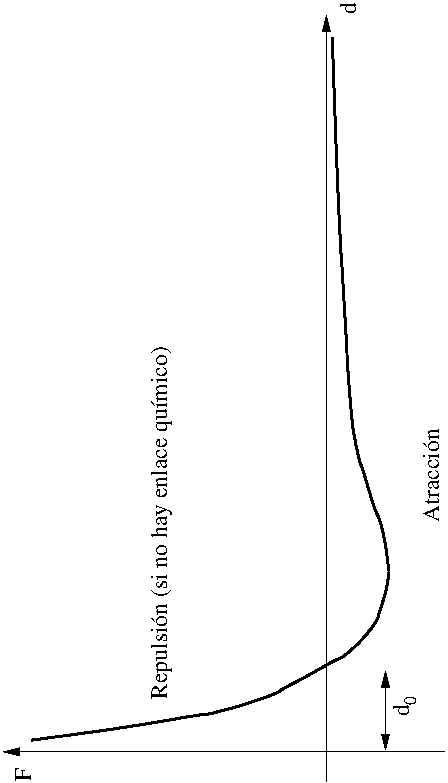
\includegraphics[scale=1,angle=270]{TeX_files/chapter01-Introduccion/fuerzas_molec.pdf}
	\caption{Fuerzas intermoleculares}
	
\end{figure}

En $d_0$, se produce un equilibrio estable.

Para la mayoria de las mol\'eculas, $d_0$ es del orden de  $3-4\cdot10^{-10}$ metros.

Para l\'{\i}quidos, la distancia entre mol\'eculas es, aproximadamente, $d_0$. P.e., para el agua:

$$
\rho \approx 1000 \, \textrm{Kg}/\textrm{m}^3
$$
$$
\textrm{Peso molecular} \approx 0.018 \, \textrm{Kg}/\textrm{mol} \Rightarrow
m = 3.0 \cdot 10^{-26} \, \textrm{Kg}/\textrm{molecula}
$$
$$
V_m = \frac{3.0 \cdot 10^{-26} \, \textrm{Kg}/\textrm{molecula}}{1000 \, \textrm{Kg}/\textrm{m}^3}
=3.0 \cdot 10^{-29} \, \textrm{m}^3
$$
$$
V_m = \frac{4}{3} \pi R^3 \Rightarrow R \approx 1.9 \cdot 10^{-10} \, \textrm{m}
$$

Para los gases, la distancia es mucho mayor (Ejercicio: calcular $d$ para el aire).

As\'{\i}, las fuerzas entre las mol\'eculas de un gas son atractivas y muy d\'ebiles. Estas mol\'eculas
flotan por el espacio sin pr\'acticamente ninguna interacci\'on excepto las colisiones.

\section{Hipótesis del medio continuo}

Todos los materiales est\'an formados por mol\'eculas. Las propiedades del material no estan distribuidas
uniformemente. Si la escala de observaci\'on es lo bastante peque\~na, la composici\'on molecular del material
debe tenerse en cuenta (hablamos entonces de {\em Mec\'anica Estad\'{\i}stica}).

Sin embargo, en {\em Mec\'anica de Fluidos}, se habla normalmente de la densidad, la temperatura, la velocidad,
como una \textcolor{red}{distribuci\'on uniforme de estas propiedades}, sin considerar la naturaleza discreta de la materia. Es
normal hablar de "diferenciales de volumen". Sin embargo, estos diferenciales no son los mismos que los usados
en C\'alculo Infinitesimal. Son volumenes finitos, pero

\begin{itemize}
	\item lo suficientemente grandes como para albergar un n\'umero enorme de mol\'eculas, de forma que las fluctuaciones en las propiedades se anulen entre s\'{\i}, y
	\item lo suficientemente peque\~nos como para que la propiedad pueda ser considerada \em{local}.
\end{itemize}

Batchelor \cite{Batchelor1997} lo describe muy bien con una figura parecida a esta:
\begin{center}
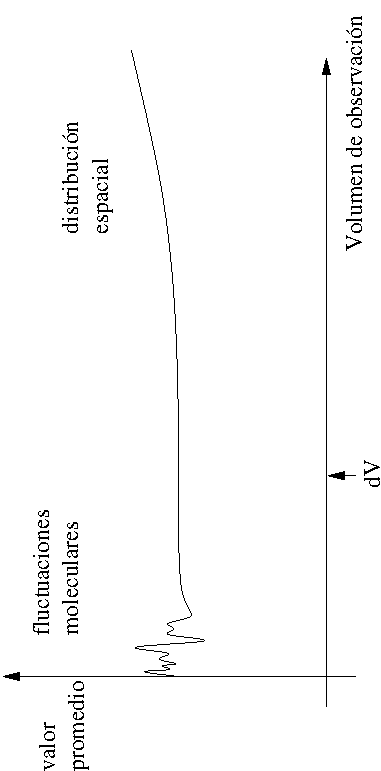
\includegraphics[scale=1,angle=270]{TeX_files/chapter01-Introduccion/difer_vol.pdf}
\end{center}

\section{Propiedades de los fluidos}
\begin{itemize}
	\item \textbf{Propiedades mec\'anicas}
	\begin{itemize}
		\item{\textcolor{red}{densidad - volumen espec\'{\i}fico}}
		$$
		\rho = \frac{m}{V} \qquad ; \qquad \left[\rho\right] = \frac{\textrm{Kg}}{\textrm{m}^3}
		$$
		$$
		v = \frac{1}{\rho} = \frac{V}{m} \qquad ; \qquad \left[v\right] = \frac{\textrm{m}^3}{\textrm{Kg}}
		$$
		\item{\textcolor{red}{M\'odulo de elasticidad} (isot\'ermico)}
		$$
		\beta_T = -v \left(\deriv{p}{v}\right)_T = \rho \left(\deriv{p}{\rho}\right)_T \qquad ; \qquad \left[\beta_T\right] = \textrm{Pa}
		$$
		
		Dado que, \textit{para un gas ideal a temperatura constante}, $\rho \propto p$, tenemos que $\beta_T = p$.
		
		Para una variaci\'on de presi\'on $\Delta p$, la variaci\'on relativa de densidad se puede calcular mediante
		
		$$
		\frac{\Delta \rho}{\rho} = \frac{\Delta p}{\beta_T}
		$$
		
		
		\begin{quotation}
			\textbf{Criterio de compresibilidad} : Todos los fluidos son compresibles, en mayor o menor grado.
			Es importante saber en qu\'e condiciones  un fluido podr\'a ser considerado compresible y cu\'ando no. Supongamos que es considerado compresible si $\frac{\Delta \rho}{\rho} \leq 0.01$. Entonces,
			$$
			\frac{\Delta p}{\beta_T} \lessapprox 0.01.
			$$
			
			Como veremos m\'as adelante, se puede relacionar $\Delta p$ con la velocidad de flujo,
			$$
			\Delta p \sim \frac{1}{2} \rho u^2,
			$$
			de forma que un fluido con velocidad $u$ se puede considerar incompresible si
			$$
			\frac{\rho u^2}{\beta_T} \lessapprox 0.02.
			$$
			
			Como ejemplo, consideremos el aire a presi\'on atmosf\'erica, $ \beta_T = p = 10^5 \,\textrm{Pa}$,
			$\rho \approx 1.2 \,\frac{\textrm{Kg}}{\textrm{m}^3}$.
			
			$$ u^2 \lessapprox \frac{0.02 \beta_T}{\rho} = \frac{0.02 \cdot 10^5}{1.2} = 1.66 \cdot 10^3 \textrm{m}^2/\textrm{s}^2$$
			$$ \Rightarrow u \approx 40 \, \textrm{m/s} $$
			
			\subsection*{Ejercicio} 
			Para el agua, a $20^\circ C$ y presi\'on atmosf\'erica, $\beta_T \approx \unit[2.2\times 10^9]{Pa}$
			y $\rho \approx \unit[1000]{Kg/m^3}$.
			Calcular para qu\'e orden de magnitud de velocidad de flujo el agua debe empezar a considerarse compresible.
		\end{quotation}
		
		\item{\textcolor{red}{Viscosidad}}
		
		Si un fluido fluye en la direcci\'on $x$, de forma ordenada, por capas, aumentando la velocidad en la direcci\'on
		$z$, como muestra la figura,
		
		\begin{center}
			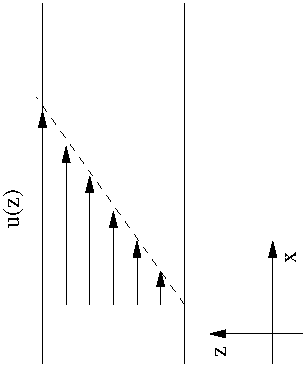
\includegraphics[scale=1,angle=270]{TeX_files/chapter01-Introduccion/u_z.pdf}
		\end{center}
		
		se produce un intercambio de cantidad de movimiento entre capas que tiende a frenar las m\'as r\'apidas y acelerar las m\'as lentas. Es decir, se produce un \textit{esfuerzo tangencial}. En muchos casos, \'este esfuerzo es proporcional al gradiente de velocidades, y a la constante de proporcionalidad se le denomina \textit{\textcolor{red}{viscosidad din\'amica}}, $\mu$. Ésta es la conocida como \textbf{Ley de Newton de la viscosidad}.
		
		\begin{equation}
			\tau = \mu \dparc{u}{z} \qquad ; \qquad \left[\mu\right] = \textrm{Pa}\cdot\textrm{s}
		\end{equation}
		
		
		La \textit{\textcolor{red}{viscosidad cinem\'atica}} se define como
		$$
		\nu = \frac{\mu}{\rho} \qquad ; \qquad \left[\nu\right] = \frac{\textrm{m}^2}{s}
		$$
		
		Ampliaremos el concepto de viscosidad en el tema siguiente.
		
	\end{itemize}
	\item {\textbf{Propiedades termodin\'amicas}}
	
	\textcolor{red}{entalp\'{\i}a}
	$$ h = u + \frac{p}{\rho} = u + p v \qquad ; \qquad \left[h\right] = \left[u\right] = \frac{\textrm{J}}{\textrm{Kg}},
	$$
	
	\textcolor{red}{calor espec\'{\i}fico}
	\begin{eqnarray*}
		c_v = \left(\dparc{q}{T}\right)_v = \dparc{u}{T} & \textrm{a volumen constante} \\
		c_p = \left(\dparc{q}{T}\right)_p = \dparc{h}{T} & \textrm{a presi\'on constante}
	\end{eqnarray*}
	$$
	\left[ c_p \right] = \left[ c_v \right] = \frac{\textrm{J}}{\textrm{Kg}\cdot\textrm{K}}
	$$
	
	La relaci\'on entre ambos coeficientes es:
	$$
	c_p = c_v + \dparc{p v}{T}
	$$
	
	Para un gas perfecto,
	$$ pv = R^\prime T  \Rightarrow \dparc{pv}{T} = R^\prime $$
	$$ \Rightarrow c_p = c_v + R^\prime $$,
	donde $R^\prime = \frac{R}{M}$.
	
	El cociente entre los dos coeficientes se denomina \textit{\textcolor{red}{exponente adiab\'atico}},
	$$
	\gamma = \frac{c_p}{c_v}.
	$$
	
	\textcolor{red}{coeficiente de expansi\'on t\'ermica}
	
	Normalmente,  $\uparrow T \Rightarrow \uparrow v \, (\Rightarrow \downarrow \rho)$.
	
	$$
	\alpha = \frac{1}{v}\deriv{v}{T} = - \frac{1}{\rho} \deriv{\rho}{T} \qquad; \qquad \left[ \alpha \right] = \textrm{K}^{-1}
	$$
	
	Para agua en condiciones normales, $\alpha \approx 1.5\cdot10^{-4} \,\textrm{K}^{-1}$.
	
	Consideremos un gas perfecto, a presi\'on constante,
	$$
	\alpha_p = -\frac{1}{\rho}\left( \dparc{\rho}{T}\right)_p,
	$$
	como $\rho = \frac{p}{R^\prime T}$,
	$$\left(\dparc{\rho}{T}\right)_p = -\frac{p}{R^\prime T^2} \qquad \Rightarrow \alpha_p = \frac{1}{T}$$	
\end{itemize}

\section{Fuerzas sobre fluidos}
\subsection{Fuerzas de superficie}

Act\'uan sobre el contorno de un  volumen determinado de fluido.

Se crean por contacto bien del mismo fluido, un fluido diferente o un s\'olido.

Dada una superficie $\delta \vec S$, y una fuerza superficial $\delta \vec F$ actuando sobre ella, \'esta se
puede descomponer en una componente normal y una componente tangencial.

\begin{center}
	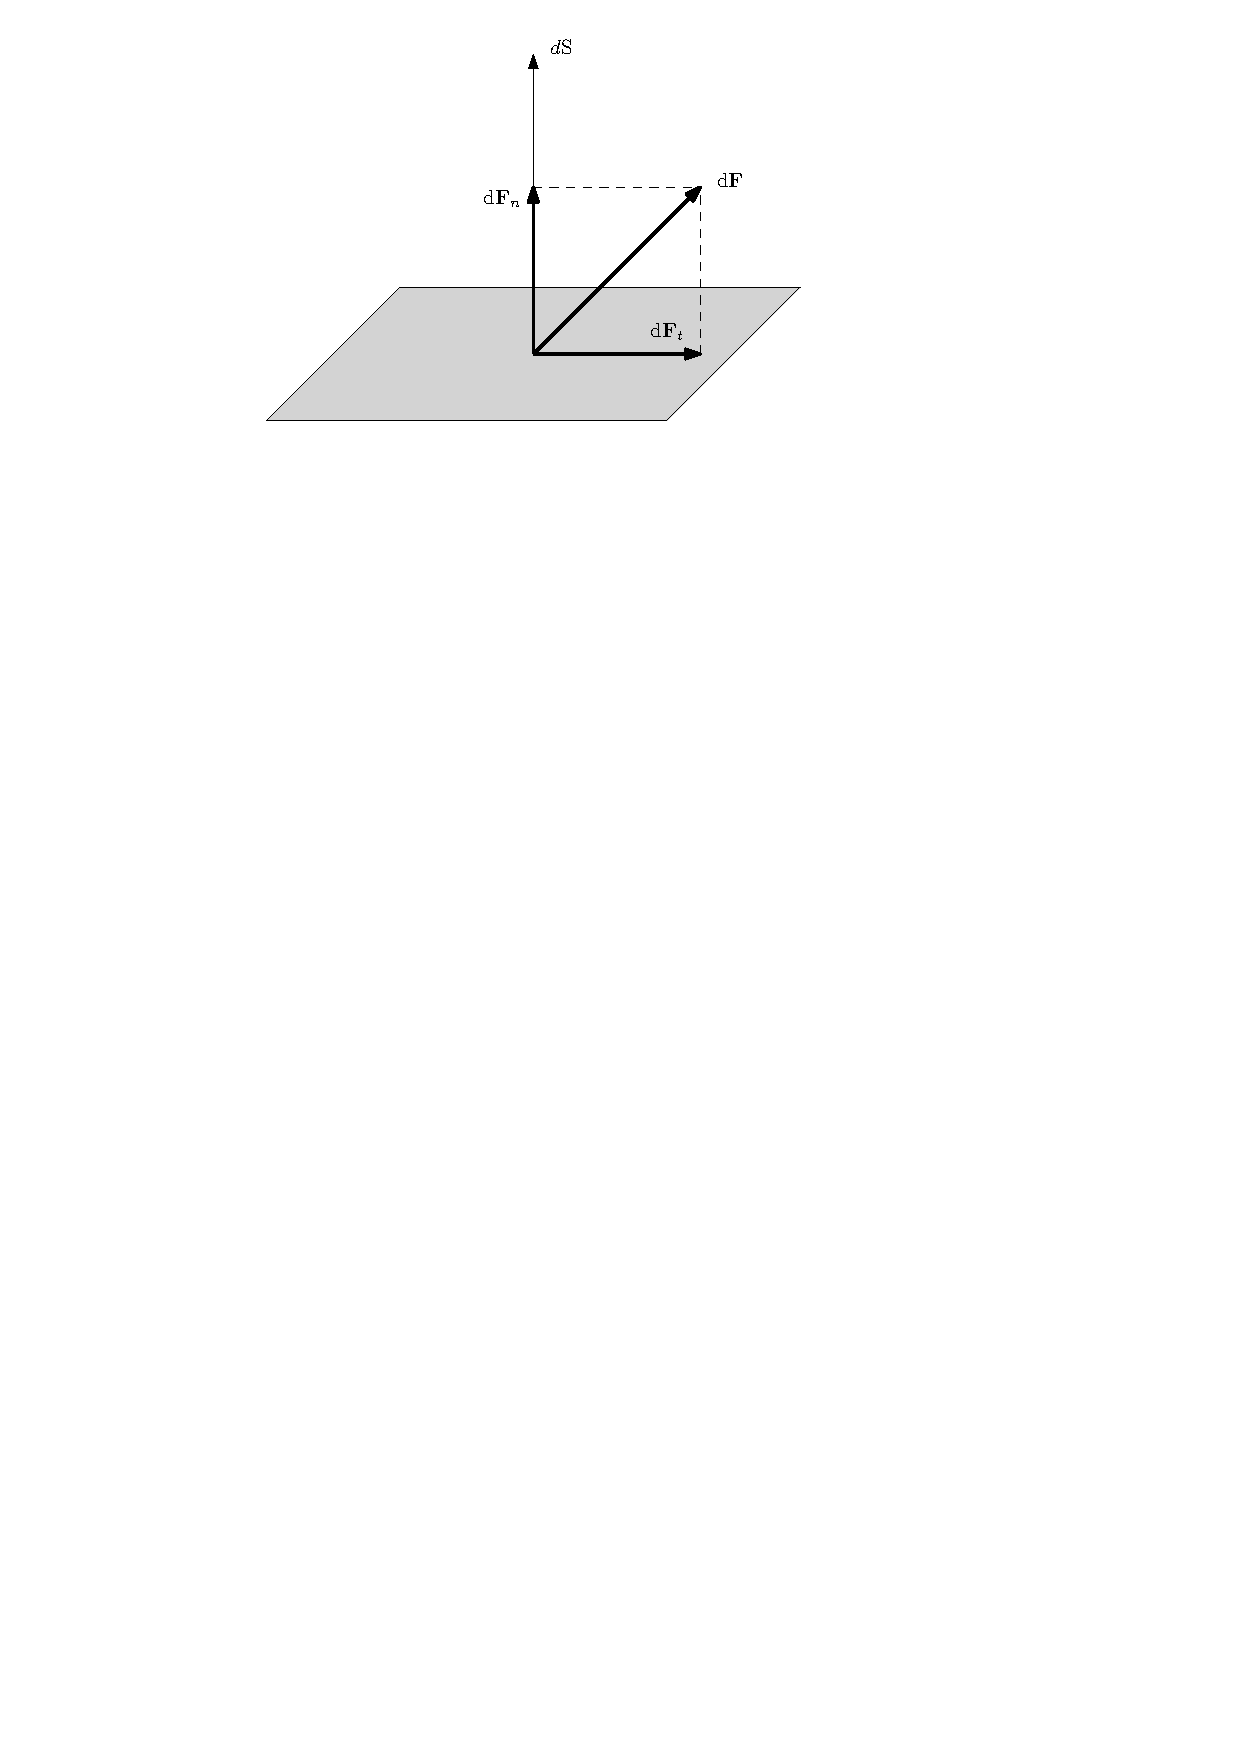
\includegraphics{TeX_files/chapter01-Introduccion/dS.pdf}
\end{center}

Definici\'on de tensi\'on o esfuerzo:

%\begin{center}
	\begin{tabular}{ll}
		\textcolor{blue}{esfuerzo normal} : & \begin{minipage}{10cm}$$\sigma = \lim_{\delta \vec S \rightarrow 0} \frac{\delta \vec F_n}{\delta \vec S}$$\end{minipage} \\
		\textcolor{blue}{esfuerzo tangencial} : & \begin{minipage}{10cm}$$\tau = \lim_{\delta \vec S \rightarrow 0} \frac{\delta \vec F_t}{\delta \vec S}$$ \end{minipage}\\
	\end{tabular}
%\end{center}

\begin{description}
	\item[$\sigma_i$ :] esfuerzo normal aplicado sobre una superficie normal al eje $i$ (y, por lo tanto, paralelo al eje $i$)
	\item[$\tau_{ij}$ :] esfuerzo tangencial aplicado sobre una superficie normal al eje $i$, y en la direcci\'on del eje $j$
\end{description} 

\begin{center}
%	\tikzstyle{isometric}=[x={(0.710cm,-0.410cm)},y={(0cm,0.820cm)},z={(-0.710cm,-0.410cm)}]
\tikzstyle{dimetric} =[x={(0.935cm,-0.118cm)},y={(0cm,0.943cm)},z={(-0.354cm,-0.312cm)}]
\tikzstyle{dimetric2}=[x={(0.935cm,-0.118cm)},z={(0cm,0.943cm)},y={(+0.354cm,+0.312cm)}]
\tikzstyle{trimetric}=[x={(-0.926cm,0.207cm)},y={(0cm,0.837cm)},z={(0.378cm,0.507cm)}]

\begin{tikzpicture}[trimetric]
	\coordinate (O) at (0,0,0);
	\draw[-stealth] (0,0,0) -- (6,0,0) node[above]{$x$};
	\draw[-stealth] (0,0,0) -- (0,6,0) node[above]{$y$};
	\draw[-stealth] (0,0,0) -- (0,0,6) node[above]{$z$};
	\draw[fill=gray!30] (0,0,0) -- (0,4,0) -- (0,4,4) -- (0,0,4)-- cycle;	
	\draw (0,0,0) -- (4,0,0) -- (4,4,0) -- (0,4,0)-- cycle;
	\draw (0,0,0) -- (0,0,4) -- (4,0,4) -- (4,0,0)-- cycle;
	\draw[fill=gray!30] (4,0,0) -- (4,4,0) -- (4,4,4) -- (4,0,4)-- cycle;	
	\draw (0,0,4) -- (4,0,4) -- (4,4,4) -- (0,4,4)-- cycle;
	\draw (0,4,0) -- (0,4,4) -- (4,4,4) -- (4,4,0)-- cycle;
%
	\draw[-stealth,thick] (0,2,2) -- (-1,2,2) node[above ]{$\sigma_x$};
	\draw[-stealth,thick] (0,2,2) -- (0,1,2) node[right]{$\tau_{xy}$};
	\draw[-stealth,thick] (0,2,2) -- (0,2,1) node[above=2mm]{$\tau_{xz}$};
%
	\draw[-stealth,thick] (4,2,2) -- (5,2,2) node[left=2mm]
					{$\sigma_x+\frac{\partial \sigma_x}{x} \textrm{d}x$};
	\draw[-stealth,thick] (4,2,2) -- (4,3,2) node[above left]
					{$\tau_{xy}+\frac{\partial \tau_{xy}}{x} \textrm{d}x$};
	\draw[-stealth,thick] (4,2,2) -- (4,2,3) node[right]
					{$\tau_{xz}+\frac{\partial \tau_{xz}}{x} \textrm{d}x$};
\end{tikzpicture}
\tikzstyle{isometric}=[x={(0.710cm,-0.410cm)},y={(0cm,0.820cm)},z={(-0.710cm,-0.410cm)}]
\tikzstyle{dimetric} =[x={(0.935cm,-0.118cm)},y={(0cm,0.943cm)},z={(-0.354cm,-0.312cm)}]
\tikzstyle{dimetric2}=[x={(0.935cm,-0.118cm)},z={(0cm,0.943cm)},y={(+0.354cm,+0.312cm)}]
\tikzstyle{trimetric}=[x={(-0.926cm,0.207cm)},y={(0cm,0.837cm)},z={(0.378cm,0.507cm)}]

\begin{tikzpicture}[trimetric]
	\coordinate (O) at (0,0,0);
	\draw[-stealth] (0,0,0) -- (6,0,0) node[above]{$x$};
	\draw[-stealth] (0,0,0) -- (0,6,0) node[above]{$y$};
	\draw[-stealth] (0,0,0) -- (0,0,6) node[above]{$z$};
	\draw[fill=gray!30] (0,0,0) -- (0,4,0) -- (0,4,4) -- (0,0,4)-- cycle;	
	\draw (0,0,0) -- (4,0,0) -- (4,4,0) -- (0,4,0)-- cycle;
	\draw (0,0,0) -- (0,0,4) -- (4,0,4) -- (4,0,0)-- cycle;
	\draw[fill=gray!30] (4,0,0) -- (4,4,0) -- (4,4,4) -- (4,0,4)-- cycle;	
	\draw (0,0,4) -- (4,0,4) -- (4,4,4) -- (0,4,4)-- cycle;
	\draw (0,4,0) -- (0,4,4) -- (4,4,4) -- (4,4,0)-- cycle;
%
	\draw[-stealth,thick] (0,2,2) -- (-1,2,2) node[above ]{$\sigma_x$};
	\draw[-stealth,thick] (0,2,2) -- (0,1,2) node[right]{$\tau_{xy}$};
	\draw[-stealth,thick] (0,2,2) -- (0,2,1) node[above=2mm]{$\tau_{xz}$};
%
	\draw[-stealth,thick] (4,2,2) -- (5,2,2) node[left=2mm]
					{$\sigma_x+\frac{\partial \sigma_x}{x} \textrm{d}x$};
	\draw[-stealth,thick] (4,2,2) -- (4,3,2) node[above left]
					{$\tau_{xy}+\frac{\partial \tau_{xy}}{x} \textrm{d}x$};
	\draw[-stealth,thick] (4,2,2) -- (4,2,3) node[right]
					{$\tau_{xz}+\frac{\partial \tau_{xz}}{x} \textrm{d}x$};
\end{tikzpicture}
\end{center}

Sobre el volumen $\text{d} V$ act\'ua una fuerza, debida a los esfuerzos superficiales cuya componente $x$ es
\begin{multline}
	\dif F_x = -\sigma_x  \dif y \dif z + \left(\sigma_x + \dparc{\sigma_x}{x} \dif x\right) \dif y \dif z - \tau_{yx} \dif x \dif z + \left(\tau_{yx} + \dparc{\tau_{yx}}{y}\right) \dif x \dif z \\
	- \tau_{zx} \dif x \dif y + \left(\tau_{zx} + \dparc{\tau_{zx}}{z}\right) \dif x \dif y
	= \dparc{\sigma_x}{x} \dif x \dif y \dif z + \dparc{\tau_{yx}}{y} \dif x \dif y \dif z + \dparc{\tau_{zx}}{z}
	\dif x \dif y \dif z
\end{multline}
De la misma forma:
\begin{eqnarray}
	\dif F_y = \dparc{\sigma_y}{y} \dif x \dif y \dif z + \dparc{\tau_{xy}}{x} \dif x \dif y \dif z + \dparc{\tau_{zy}}{z} \dif x \dif y \dif z \\
	\dif F_z = \dparc{\sigma_z}{z} \dif x \dif y \dif z + \dparc{\tau_{xz}}{x} \dif x \dif y \dif z + \dparc{\tau_{yz}}{y} \dif x \dif y \dif z
\end{eqnarray}

La fuerza por unidad de volumen, debida a los esfuerzos superficiales es entonces
\begin{eqnarray*}
	\vec f = \deriv{\vec F}{V} = \left( \dparc{\sigma_x}{x} + \dparc{\tau_{yx}}{y} + \dparc{\tau_{zx}}{z}\right) \vec \imath \\
	+ \left( \dparc{\tau_{xy}}{x} + \dparc{\sigma_y}{y} +  \dparc{\tau_{zy}}{z} \right) \vec \jmath \\
	+ \left( \dparc{\tau_{xz}}{x}  +  \dparc{\tau_{yz}}{y} + \dparc{\sigma_z}{z} \right) \vec k
\end{eqnarray*}
que se expresa de forma abreviada como
\begin{equation}
	 \vec f = \vec \nabla \vec {\vec \tau}
\end{equation}
donde $\vec {\vec \tau}$ es el \textcolor{red}{tensor de tensiones} (stress tensor)
\begin{equation}
	\vec{\vec{\tau}} =
	\left(
	\begin{array}{ccc}
		\sigma_x & \tau_{xy} & \tau_{xz} \\
		\tau_{yx} & \sigma_y & \tau_{yz} \\
		\tau_{zx} & \tau_{zy} & \sigma_z
	\end{array}\right)
\end{equation}

\subsection{Fuerzas m\'asicas}
Act\'uan a distancia

Son debidas a campos de fuerza (gravitacional, electromagn\'etico, \ldots)

Fluido el\'ectricamente cargado : plasma
\begin{itemize}
	\item Electrohidrodin\'amica
	\item Magnetohidrodin\'amica
\end{itemize}

Caso m\'as com\'un: s\'olo campo gravitacional
$$\vec f_g = \rho \vec g$$

\subsection{Fuerzas lineales (tensi\'on superficial)}
En la interfase de separaci\'on entre dos l\'iquidos reside una cantidad de energ\'{\i}a, correspondiente
a la interacci\'on entre moleculas muy pr\'oximas a la superficie de separaci\'on

Esta energ\'{\i}a es proporcional al \'area de la interfase.
\begin{equation}
	 E_s = \sigma S
\end{equation} 

El par\'ametro $\sigma$ recibe el nombre de \textcolor{blue}{tensi\'on superficial} y tiene unidades de fuerza por
unidad de longitud. Esta fuerza es tangente a la superficie, y normal a la l\'{\i}nea de aplicaci\'on.

El valor de $\sigma$ depende de la naturaleza de los materiales que separa la interfase y de su estado termodin\'amico.

P.e. para la interfase entre agua y aire a $20^\circ C$, $\sigma~=~72.8\cdot10^{-3}~\text{N/m}$


\begin{center}
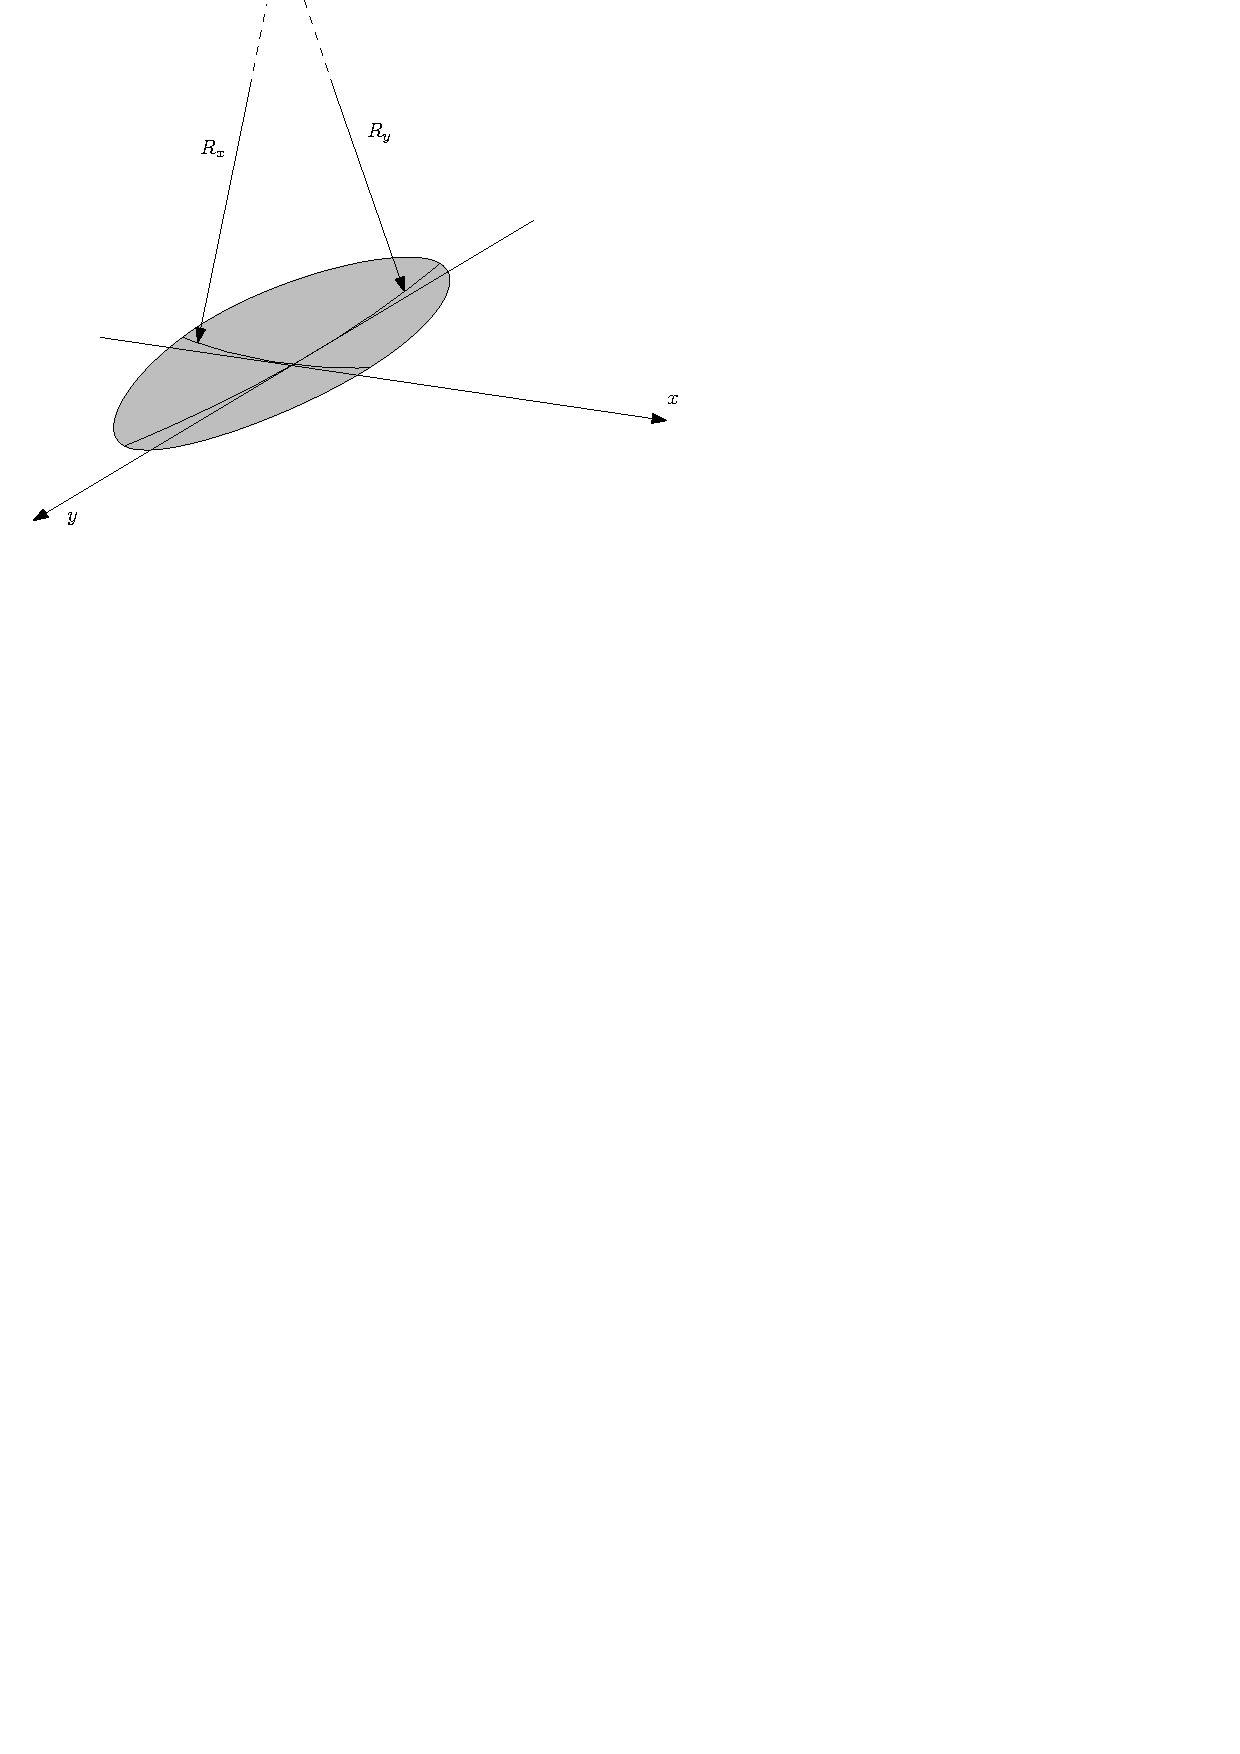
\includegraphics{TeX_files/chapter01-Introduccion/YoungLaplace}
\end{center}
Se puede demostrar (ver \cite{Batchelor1997}) que la tensi\'on provocada en la superfice es equivalente a una diferencia
de presi\'on, como indica la \href{https://es.wikipedia.org/wiki/Ley_de_Laplace}{\textbf{ley de Young-Laplace}}
\begin{equation}
	\Delta p = \sigma\left(\frac{1}{R_x}+\frac{1}{R_y}\right)
\end{equation}


Si los dos radios de curvatura son iguales, ($R_x=R_y=R$, casquete esférico), esta expresión se reduce a 
 
\begin{equation}
	\Delta p = \frac{2\sigma}{R}
\end{equation}

Consideramos el caso de tres fluidos (p.e. una gota de aceite en una superficie de agua)
\begin{center}
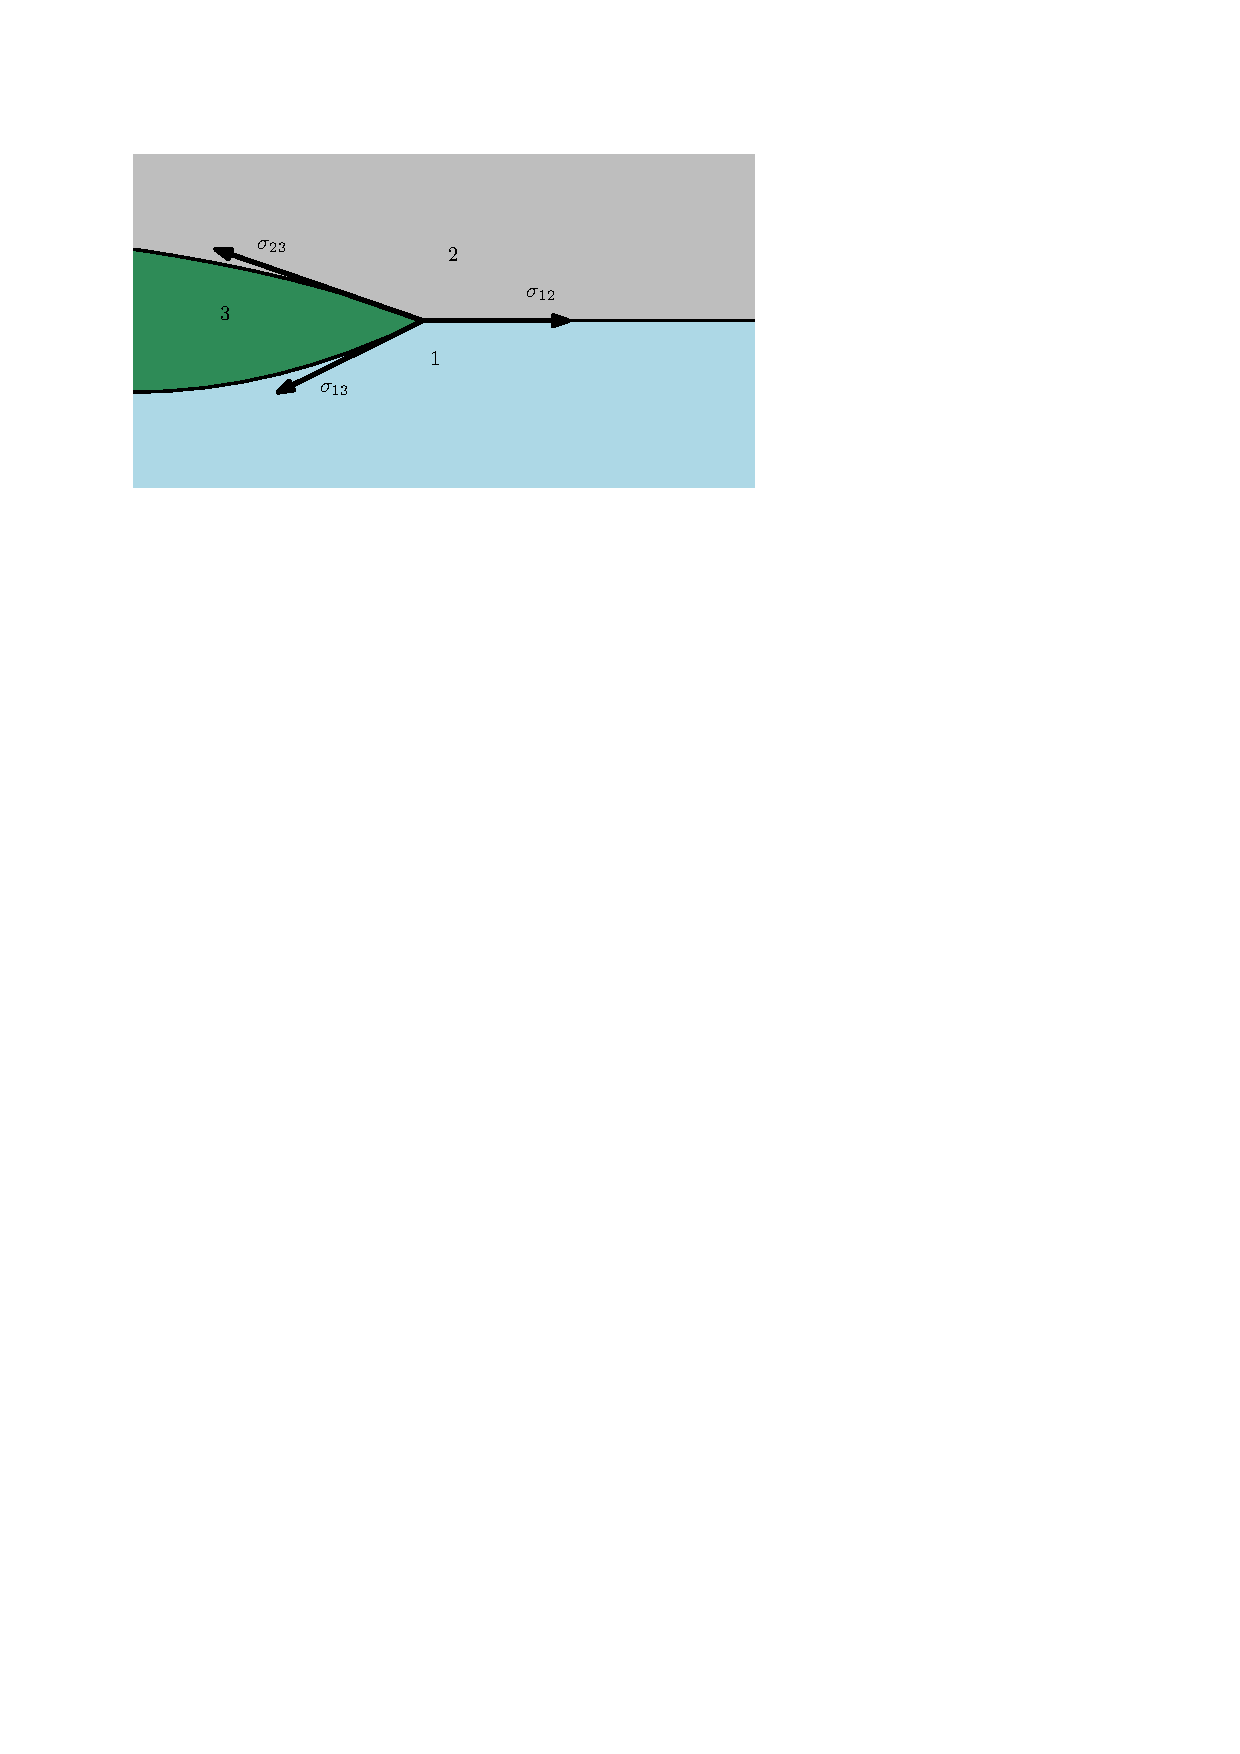
\includegraphics{TeX_files/chapter01-Introduccion/tresFluidos}
\end{center}
Si el m\'odulo de una de las tensiones es mayor que la suma de los m\'odulos de las otras dos, este sistema nunca
puede llegar al equilibrio, y el fluido se expandir\'a de forma indefinida hasta llegar al equilibrio, o tener
un grosor de tama\~no molecular.

Si uno de los materiales es un s\'olido,
\begin{center}
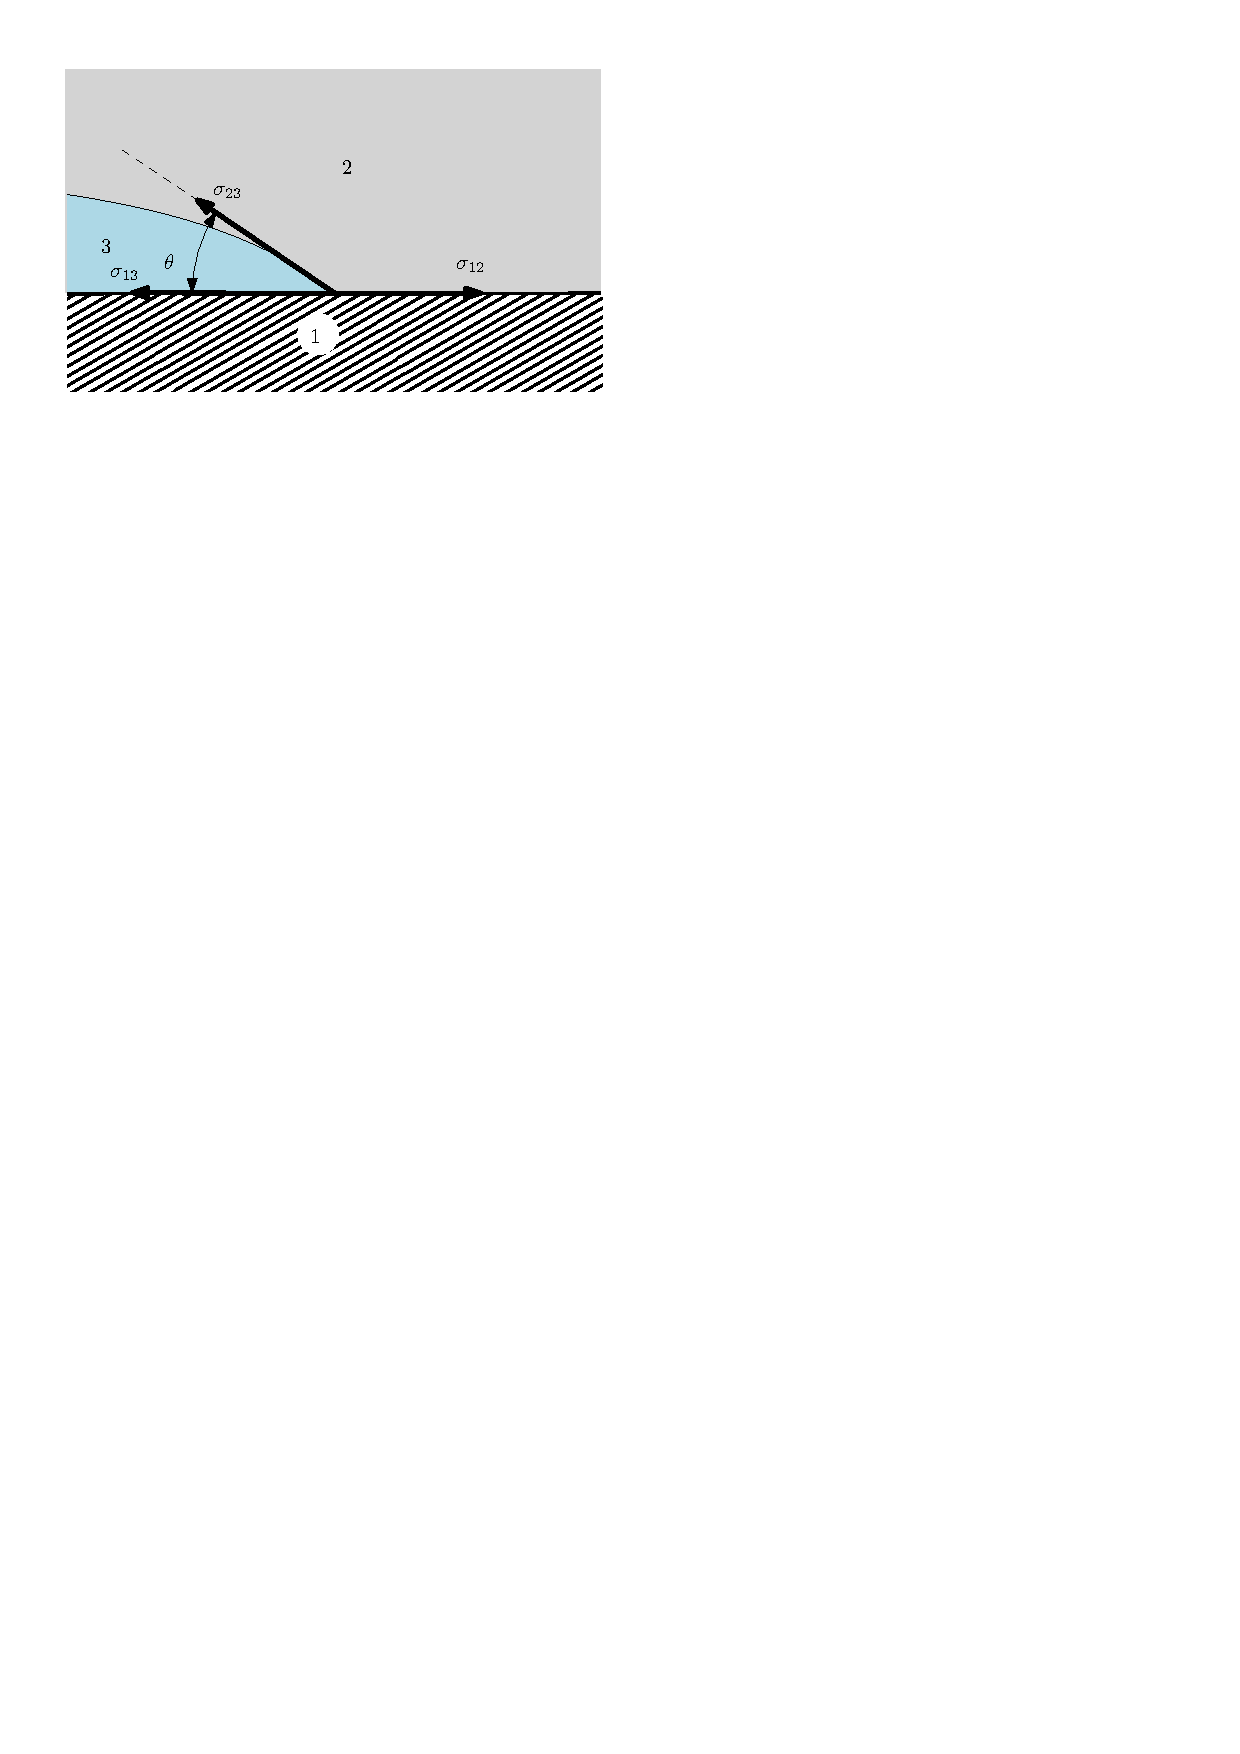
\includegraphics{TeX_files/chapter01-Introduccion/dosysolido}
\end{center}
se llega al equilibrio para
$$ \sigma_{12} = \sigma_{31} + \sigma_{23} \cos{\theta}$$
Se considera que cuanto menor es $\theta$, m\'as "moja" el fluido sobre la superficie del s\'olido.

\subsection*{Ejemplo:}
L\'{\i}quido en contacto con pared plana vertical
\begin{center}
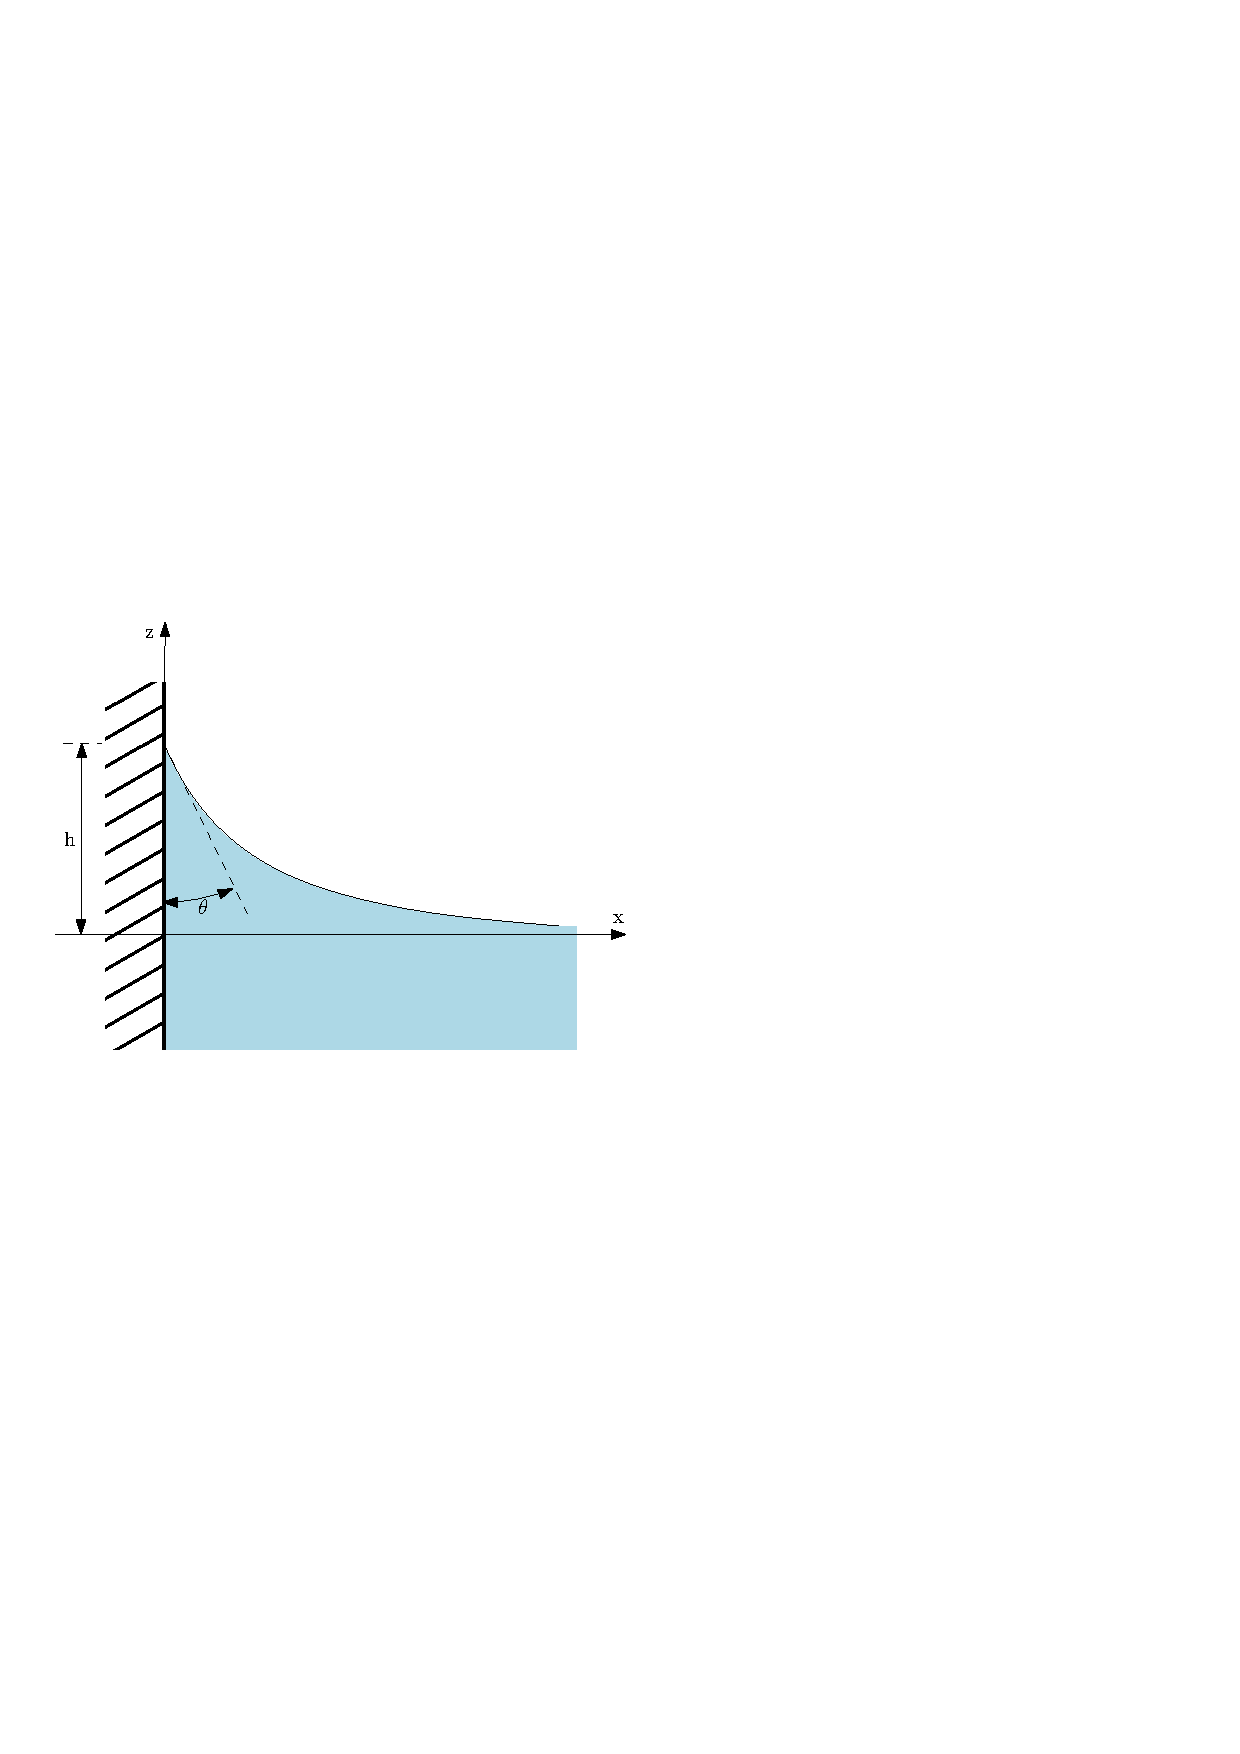
\includegraphics{TeX_files/chapter01-Introduccion/pared.pdf}
\end{center}
Forma de la interficie: $z=\zeta(x)$

En un cierto punto de la interficie, la tensi\'on superficial tiene que ser tal que compense la presi\'on de la columna de fluido. Como veremos m\'as adelante, esta es $\rho g z$, de forma que
$$
\rho g z = \sigma \frac{1}{R_1}
$$
$$
\rho g \zeta = \sigma \frac{\zeta''}{\left( 1 + \zeta'^2\right)^\frac{3}{2}}
$$
Integrando se obtiene
$$
\frac{1}{2}\frac{\rho g}{\sigma}\zeta^2 + \frac{1}{\left(1+\zeta'^2\right)^\frac{1}{2}} = K
$$
Muy lejos de la pared, se cumple que $\zeta=\zeta'=0$, de forma que $K = 1$

Por otro lado, en $x=0$, se tiene (ver figura) $\zeta=h$ y $\zeta'=-\frac{1}{\tan \theta}$, de forma que
$$
h = d \sqrt{2\left(1-\sin \theta \right)}
$$
donde $d^2=\frac{\sigma}{\rho g}$.
\chapter{Hidrostática}

\section{Ecuación fundamental de la fluidostática}

\textbf{Fluido en reposo}: No hay esfuerzos tangenciales, y la única
fuerza superficial es la presión.

Equilibrio estático: 

\begin{equation}
\vec{f}_{m}-\vec{\nabla}p=0
\end{equation}


Según el calculo diferencial, 
\[
\vec{\nabla}\times\left(\vec{\nabla}\phi\right)=0\quad\forall\phi\text{ escalar}
\]

\[
\Rightarrow\vec{\nabla}\times\vec{f_{m}}=0.
\]
 $\Rightarrow\vec{f}_{m}$ ha de ser un \emph{campo conservativo}.

\[
\dif p=\vec{f}_{m}\cdot\dif\vec{r}
\]
 Integrando sobre un determinado camino, 
\[
p\left(\vec{r}\right)=p\left(\vec{r}_{0}\right)+\int_{\vec{r}_{0}}^{\vec{r}}\vec{f}_{m}\cdot\dif\vec{r}
\]
 Nos permite calcular la presión en cualquier punto $\vec{r}$ conociendo
el valor en un punto de referencia $\vec{r}_{0}$ y el campo de fuerzas
$\vec{f}_{m}$.

Si $\vec{f}_{m}$ es conservativo 
\[
\vec{f}_{m}=-\rho\vec{\nabla}U
\]
 y, entonces, 
\[
\vec{\nabla}p=-\rho\vec{\nabla}U
\]

Si $\rho$ varia de forma arbitraria, no existen soluciones para la
ecuación , y no es posible llegar al equilibrio, $\rightarrow$ \textcolor{blue}{corrientes
convectivas}

La ecuación sólo admite soluciones cuando $\rho$ es únicamente función
de la presión, o bien es constante (fluido incompresible). 
\[
p+\rho U=cte
\]

$\rightarrow$ \textcolor{blue}{Principio de Pascal}

Hidrostática en el campo de la gravedad

\[
\vec{f}_{m}=\rho\vec{g},
\]
 con 
\[
\vec{g}=-g\vec{k}\qquad\text{donde }g=9.81\,\frac{\textrm{m}}{\textrm{s}^{2}}
\]
 y 
\[
U=gz
\]



Superficies isobáricas (superficies de igual presión), incluida la
superficie libre de los líquidos, horizontales. %

\[
\vec{\nabla}p=-\rho g\vec{k}\Rightarrow\left\{ \begin{aligned}\dparc{p}{x} & =0\\
\dparc{p}{y} & =0\\
\dparc{p}{z} & =-\rho g
\end{aligned}
\right.
\]
%

La presión es únicamente función de la coordenada $z$.

\[
\deriv{p}{z}=-\rho\,g\Rightarrow\,p_{2}-p_{1}
\]

\[
=-\int_{z_{1}}^{z_{2}}\rho\,g\,\dif z
\]
%

\subsection*{Actividad 1:}
\noindent\begin{minipage}[t]{1\columnwidth}%
\begin{itemize}
\item ¿A cuántos metros de columna de agua corresponden la presión atmosférica?
\item Si el aire fuese incompresible, con la densidad que tiene a nivel
del mar, ¿cuál debería ser la altura de la atmósfera para tener la
misma presión?
\end{itemize}
%
\end{minipage}

\section{Presión atmosférica}

La presión atmosférica disminuye con la altura. Dado que el aire es
un gas, su densidad disminuye, en general, cuando disminuye la presión,
por lo que también es menor cuando aumentamos la altura.

Necesitamos información sobre la variación de $\rho$ con $z$, o
bien con $p$.

Opción: aire gas ideal 
\[
\rho=\frac{pM}{RT}\quad\textnormal{con}\,M=28.9\,\textnormal{g/mol}.
\]
 
\begin{equation}
\Rightarrow\,\frac{\dif p}{p}=-\frac{Mg}{RT}\dif z\label{eq:general}
\end{equation}



Sin considerar la variación de $g$ con la altura: 
\begin{itemize}
\item \textcolor{blue}{Atmósfera isoterma:} 
\[
\int_{p_{0}}^{p}\frac{\dif p}{p}=-\int_{0}^{z}\frac{Mg}{RT}\dif z
\]
 
\[
\ln\frac{p}{p_{0}}=-\frac{Mg}{RT}z=-\frac{\rho_{0}g}{p_{0}}z
\]
 
\begin{equation}
\Rightarrow\boxed{p=p_{0}\exp\left(-\frac{\rho_{0}g}{p_{0}}z\right)=p_{0}\exp\left(-\frac{z}{\alpha}\right)}\label{eq:isotermica}
\end{equation}
 donde 
\[
\alpha=\frac{p_{0}}{\rho_{0}g}
\]
\end{itemize}
Valores normales: 
\[
\left.\begin{aligned}\rho_{0} & =1.292\,\text{Kg}/\text{m}^{3}\\
g & =9.80665\,\text{m}/\text{s}^{2}\\
p_{0} & =760\,\text{mmHg}=101328\,\text{Pa}
\end{aligned}
\right\} \rightarrow\alpha=7997.35\,\text{m}\approx8000\,\text{m}
\]



\begin{itemize}
\item \textcolor{blue}{Atmósfera adiabática:} 
\[
\frac{p}{\rho^{\gamma}}=\frac{p_{0}}{\rho_{0}^{\gamma}}\qquad\text{con}\qquad\gamma=\frac{c_{p}}{c_{v}}=1.4\qquad\text{para aire}
\]
\end{itemize}
\[
\dif p=-g\rho\dif z=-\rho_{0}\left(\frac{p}{p_{0}}\right)^{\frac{1}{\gamma}}g\dif z
\]
 
\[
\Rightarrow\frac{\dif p}{p^{\frac{1}{\gamma}}}=-\frac{\rho_{0}}{p_{0}^{\frac{1}{\gamma}}}g\dif z
\]

\[
\int_{p_{0}}^{p}\frac{\dif p}{p^{\frac{1}{\gamma}}}=\int_{0}^{z}-\frac{\rho_{0}}{p_{0}^{\frac{1}{\gamma}}}g\dif z=-\frac{\rho_{0}}{p_{0}^{\frac{1}{\gamma}}}gz
\]


\[
\Rightarrow\frac{1}{-\frac{1}{\gamma}+1}\left.p^{-\frac{1}{\gamma}+1}\right]_{p_{0}}^{p}=-\frac{\rho_{0}}{p_{0}^{\frac{1}{\gamma}}}gz
\]

\[
\Rightarrow\frac{\gamma}{\gamma-1}\left[p^{\frac{\gamma-1}{\gamma}}-p_{0}^{\frac{\gamma-1}{\gamma}}\right]=-\frac{\rho_{0}}{p_{0}^{\frac{1}{\gamma}}}gz
\]

\[
\Rightarrow p^{\frac{\gamma-1}{\gamma}}-p_{0}^{\frac{\gamma-1}{\gamma}}=\frac{1-\gamma}{\gamma}\frac{\rho_{0}}{p_{0}^{\frac{1}{\gamma}}}gz
\]

\begin{equation}
\Rightarrow\boxed{\left(\frac{p}{p_{0}}\right)^{\frac{\gamma-1}{\gamma}}=1+\frac{1-\gamma}{\gamma}\frac{z}{\alpha}}\label{eq:adiabatica}
\end{equation}


\begin{itemize}
\item \textcolor{blue}{Atmósfera estándar:}
\end{itemize}
En realidad, la temperatura media de la atmósfera disminuye de forma
casi lineal con la altura 
\[
T=T_{0}-Bz
\]
 hasta una altura aproximada de 11000 metros (región conocida como
\textit{troposfera}). Los valores de $T_{0}$ (la temperatura a nivel
del mar) y $B$ (\textit{gradiente térmico}) varían no sólo según
el día sino también a lo largo del mismo día. Los valores estándar
usados por convenio son 
\begin{eqnarray*}
T_{0} & = & 15^{\circ}C=288.16\textnormal{K}\\
B & = & 0.0065\textnormal{K/m}
\end{eqnarray*}



\subsection*{Actividad 2:}
Integrar la ecuación (\ref{eq:general}) con esta distribución de
temperatura para obtener 
\begin{equation}
p=p_{0}\left(1-\frac{Bz}{T_{0}}\right)^{\frac{Mg}{RB}}
\end{equation}

El valor del exponente para aire es 
\[
\frac{Mg}{RB}=5.26
\]

Después de la troposfera, la temperatura se mantiene constante hasta
unos 20000 metros para empezar a aumentar de forma gradual.

Hay que tener siempre en cuenta que esta atmósfera estándar es un
valor promediado. 

\section{Fuerza de un fluido estático sobre una superficie}

\subsection{Cálculo de la fuerza}


\begin{center}
\resizebox{0.8\textwidth}{!}{\input{TeX_files/chapter02-Hidrostatica/superficie.pdftex_t}}
\par\end{center}


\[
F=\int_{S}\dif F=\int_{S}(p_{0}+\rho\,g\,h)\dif S==\int_{S}(p_{0}+\rho\,g\,y\,\sin\theta)\dif S
\]

\[
\Rightarrow\;F=p_{0}\,S+\rho\,g\,\sin\theta\int_{S}y\dif S
\]

\begin{description}
\item [{$\int_{S}y\dif S$}] : momento de primer orden de la superficie
$S$ respecto el eje $x$ $\rightarrow$ coordenada $y_{C}$ del centroide
$C$ de la forma
\end{description}
\[
y_{C}\,S=\int_{S}y\dif S\,\Rightarrow\;F=(p_{0}+\rho\,g\,y_{C}\,\sin\theta)S=(p_{0}+\rho\,g\,h_{C})S
\]

\fbox{%
\noindent\parbox[c]{1\textwidth}{%
 La fuerza ejercida sobre una superficie totalmente sumergida se puede
calcular \textbf{imaginando} que la presión que actúa es constante
en toda la superficie e igual al valor en el centroide. %
}}


\subsection{Coordenadas del punto de aplicación}


Momento de la fuerza $\vec{F}$ respecto el eje $x$: 
\[
y_{cp}F=\int_{S}y\dif F=\int_{S}y(p_{0}+\rho\,g\,y\,\sin\theta)\dif S=p_{0}\int_{S}y\dif S+\rho\,g\,\sin\theta\int_{S}y^{2}\dif S
\]
 
\[
\Rightarrow y_{cp}F=\int_{S}y\dif F=p_{0}\,y_{C}\,S+\rho\,g\,\sin\theta I_{xx}
\]
 donde $I_{xx}$ es el momento de segundo orden de la superficie $S$
respecto el eje $x$.

Nuevo sistema de coordenadas $(\xi,\eta,\zeta)$, paralelo a $(x,y,z)$
pero con origen en el centroide $C$. 
\[
I_{xx}=I_{\xi\xi}+y_{C}^{2}\,S\qquad\text{(T. de Steiner)}
\]

\[
\Rightarrow y_{cp}=y_{C}+\frac{I_{\xi\xi}}{\left(y_{C}+\frac{p_{0}}{\rho\,g\,\sin\theta}\right)S}
\]


Para $x_{cp}$: 
\[
\int_{S}x\dif F=\int_{S}x(p_{0}+\rho\,g\,y\,\sin\theta)\dif S=p_{0}\int_{S}x\dif S+\rho\,g\,\sin\theta\int_{S}xy\dif S
\]
 
\[
\Rightarrow\int_{S}x\dif F=p_{0}\,x_{C}\,S+\rho\,g\,\sin\theta I_{xy}
\]
 
\[
I_{xy}=I_{\xi\eta}+x_{C}\,y_{C}\,S\qquad\text{(T. de Steiner)}
\]
 
\[
\Rightarrow x_{cp}=x_{C}+\frac{I_{\xi\eta}}{\left(y_{C}+\frac{p_{0}}{\rho\,g\,\sin\theta}\right)S}
\]



Normalmente, $p_{0}$ (en general, la presión atmosférica) actúa por
igual en las dos caras de la superficie, 
\begin{align*}
F & =\rho\,g\,h_{C}\,S\\
x_{cp} & =x_{C}+\frac{I_{\xi\eta}}{y_{C}\,S}\\
y_{cp} & =y_{C}+\frac{I_{\xi\xi}}{y_{C}\,S}
\end{align*}

Dado que $I_{\xi\xi}$ es, por definición, una cantidad siempre positiva,
el centro de presiones se encuentra siempre por debajo del centroide.


\subsection{Fuerza sobre una superficie curva totalmente sumergida}


\begin{center}
\resizebox{!}{5cm}{\input{TeX_files/chapter02-Hidrostatica/superficie_curva.pdftex_t}}
\par\end{center}

 
\[
\begin{aligned}F_{x} & =-\int_{S}(p_{0}+\rho\,g\,h)\dif S_{x}\\
F_{y} & =-\int_{S}(p_{0}+\rho\,g\,h)\dif S_{y}
\end{aligned}
\]
 

Si proyectamos la superficie $S$ sobre los planos $x=0$ y $y=0$,
obtenemos $S_{x}$ y $S_{y}$, y podemos calcular $F_{x}$ y $F_{y}$,
así como sus puntos de aplicación.

$F_{z}$ resulta ser igual al peso total de fluido que se encuentra
\emph{por encima} de la superficie curva. La linea de acción de $F_{z}$
pasa por el centro de gravedad de la columna de fluido que hay sobre
la superficie.

Las expresiones anteriores son válidas únicamente para fluidos con
densidad constante. Si el fluido está estratificado, de forma que
hay un \textit{gradiente de densidad}, positivo hacia la dirección
vertical negativa, los cálculos se complican.


\subsection*{Actividad 3:}
Calcula la fuerza, y su punto de aplicación, que hace un embalse de agua de 50
metros de profundidad y 200 metros de ancho sobre la pared, vertical,
de la presa.


\section{Principio de Arquímedes}

\fbox{%
	\parbox{1\textwidth}{%
%\begin{quotation}
	\emph{Todo cuerpo sumergido, completa o parcialmente,
		en un fluido experimenta
		un empuje dirigido verticalmente hacia arriba, con magnitud igual al peso del
		fluido desalojado y cuya  linea de acci\'on pasa por el centro de gravedad
		del fluido desalojado}
%\end{quotation} %
}}


\begin{minipage}{0.4\textwidth}
	\begin{center}
		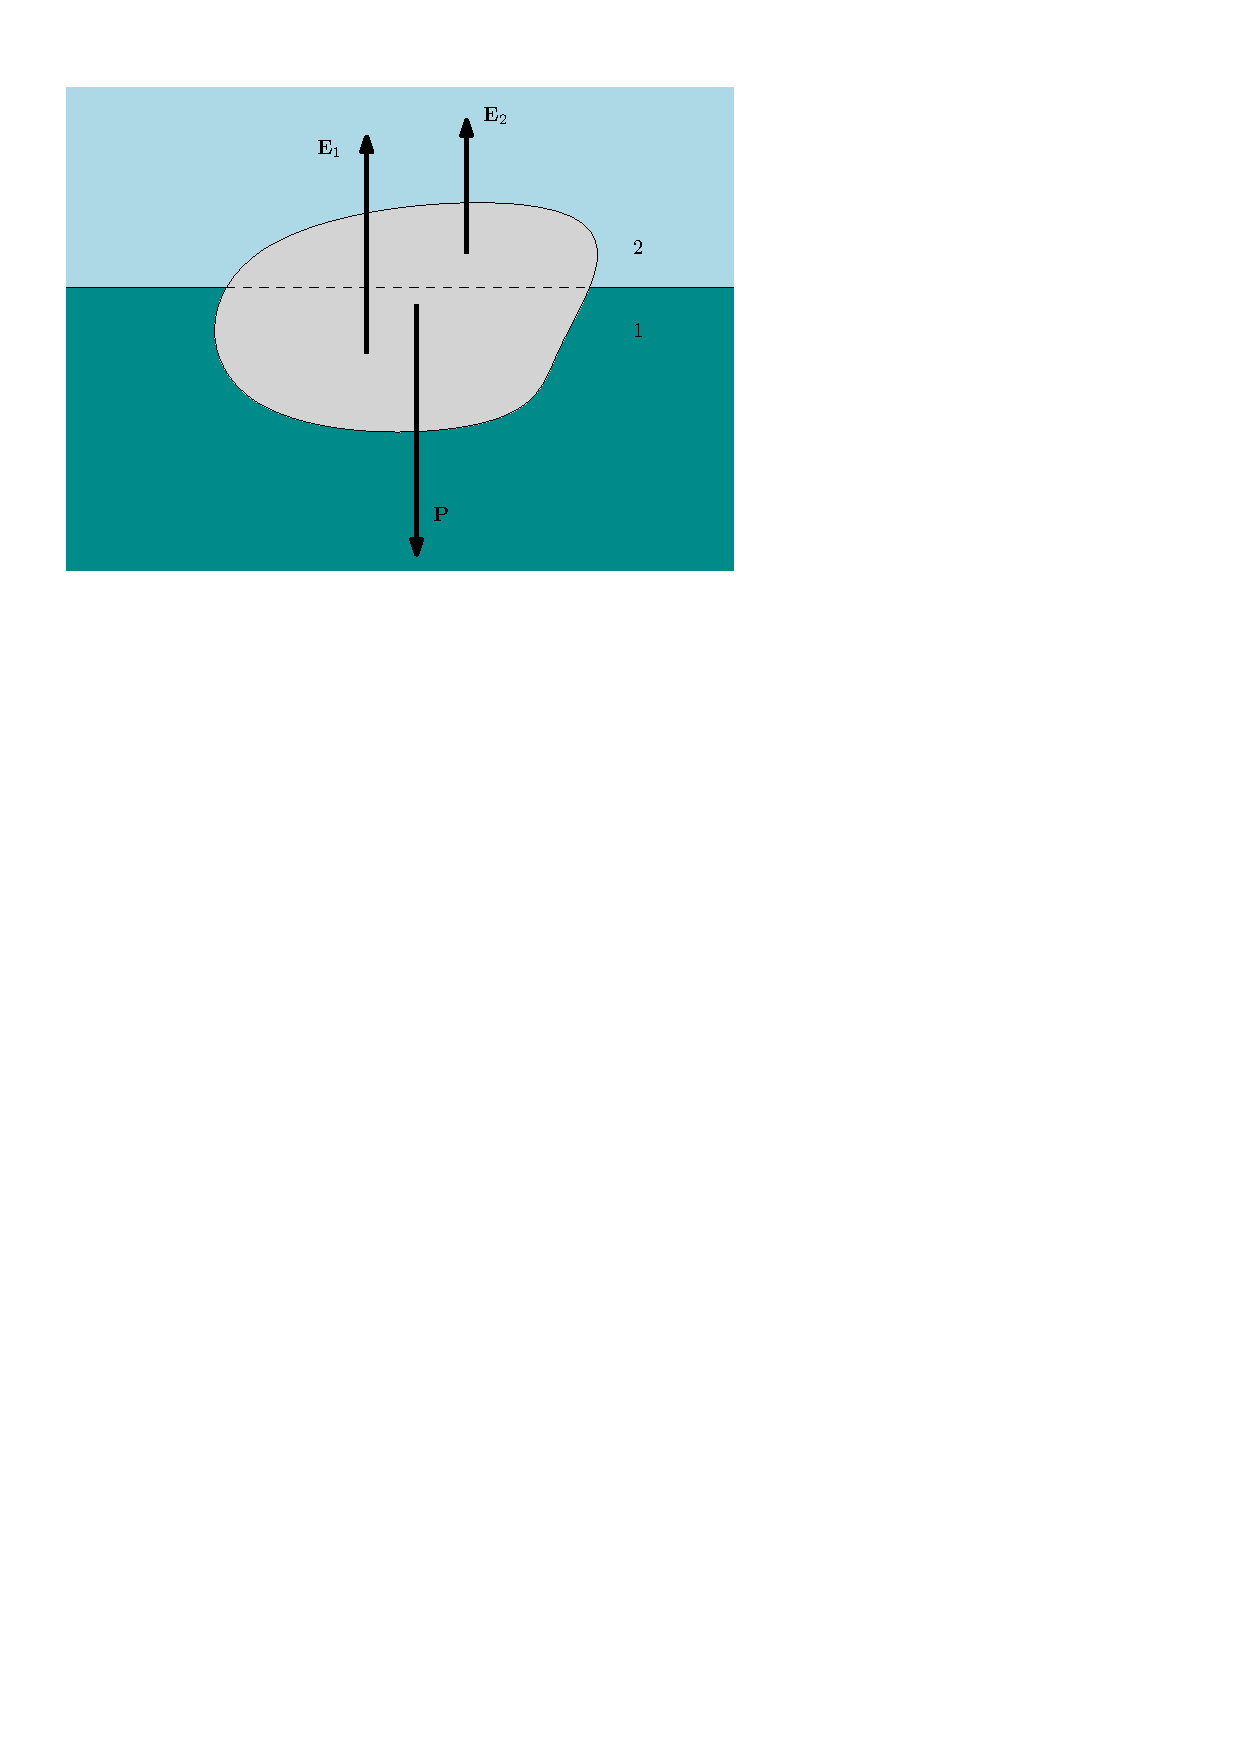
\includegraphics[width=\textwidth]{TeX_files/chapter02-Hidrostatica/arquimedes}
	\end{center}
\end{minipage}
\begin{minipage}{0.5\textwidth}
	Las lineas de acci\'on de las fuerzas de empuje y el peso no
	tienen porqu\'e coincidir, y, en este caso, se producen pares de fuerzas.
	\begin{description}
		\item[\textcolor{blue}{carena}] volumen del fluido desalojado
		\item[\textcolor{blue}{centro
			de carena} o \textcolor{blue}{centro de empuje}] centro de gravedad del fluido desalojado
	\end{description}
\end{minipage}


	El principio de Arquímedes no es, en realidad, un principio. Se puede deducir en cualquier caso simplemente calculando la integral de la presión sobre la superficie que limita el cuerpo.
	
	También se puede obervar que es la resta del peso de la columna de fluido sobre la superficie superior y sobre la superficie inferior.
	
\begin{center}
	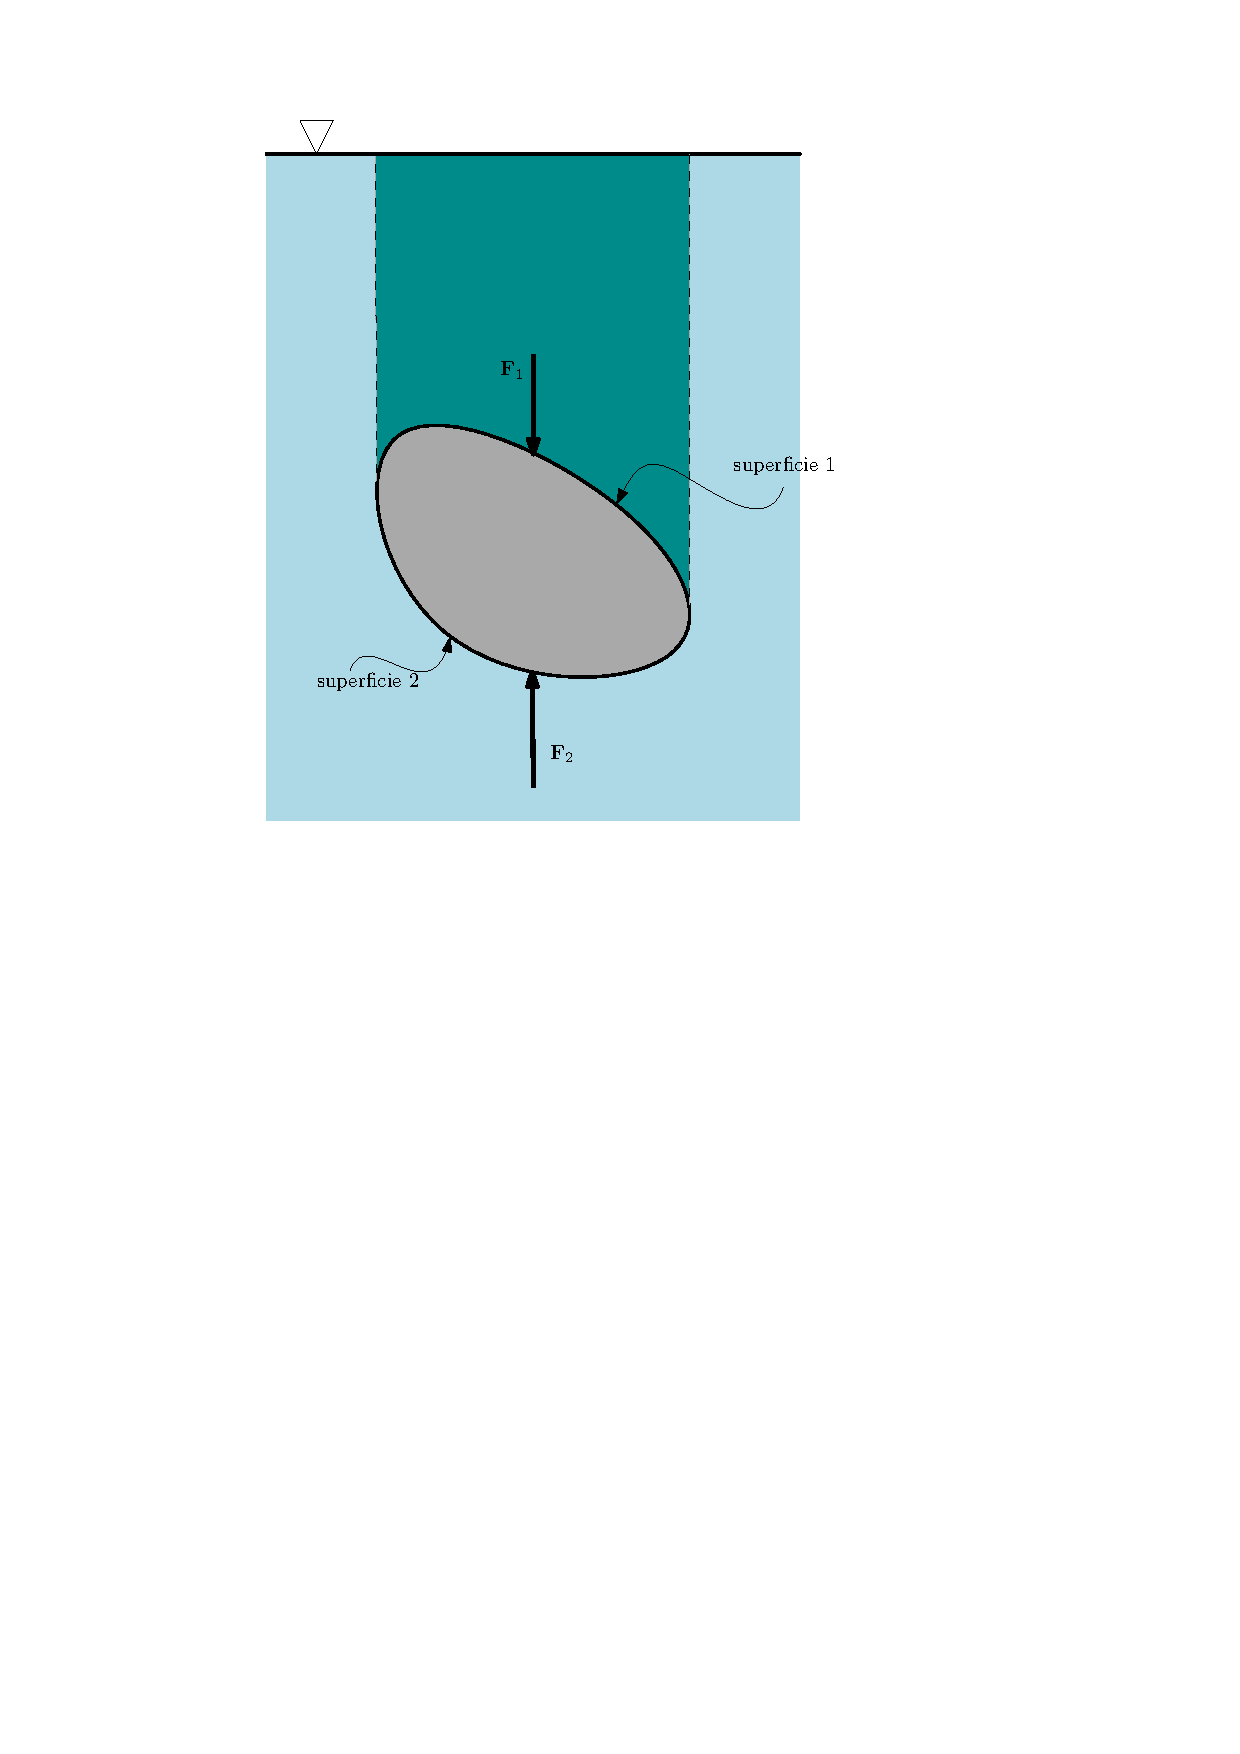
\includegraphics[width=0.5\columnwidth]{TeX_files/chapter02-Hidrostatica/arquimedes2}
\end{center}
\section{Segunda ley de Arquímedes}


	La segunda ley de Arqu\'imedes dice que \emph{un cuerpo que flota desaloja su propio peso de fluido}. 
	
	Se puede comprender observando que en la figura, el recipiente con solo fluido y el que tiene fluido y cuerpo flotando, \textbf{deben pesar lo mismo}. Pregunta: ?`C\'omo sabemos que pesan lo mismo?


	\begin{center}
		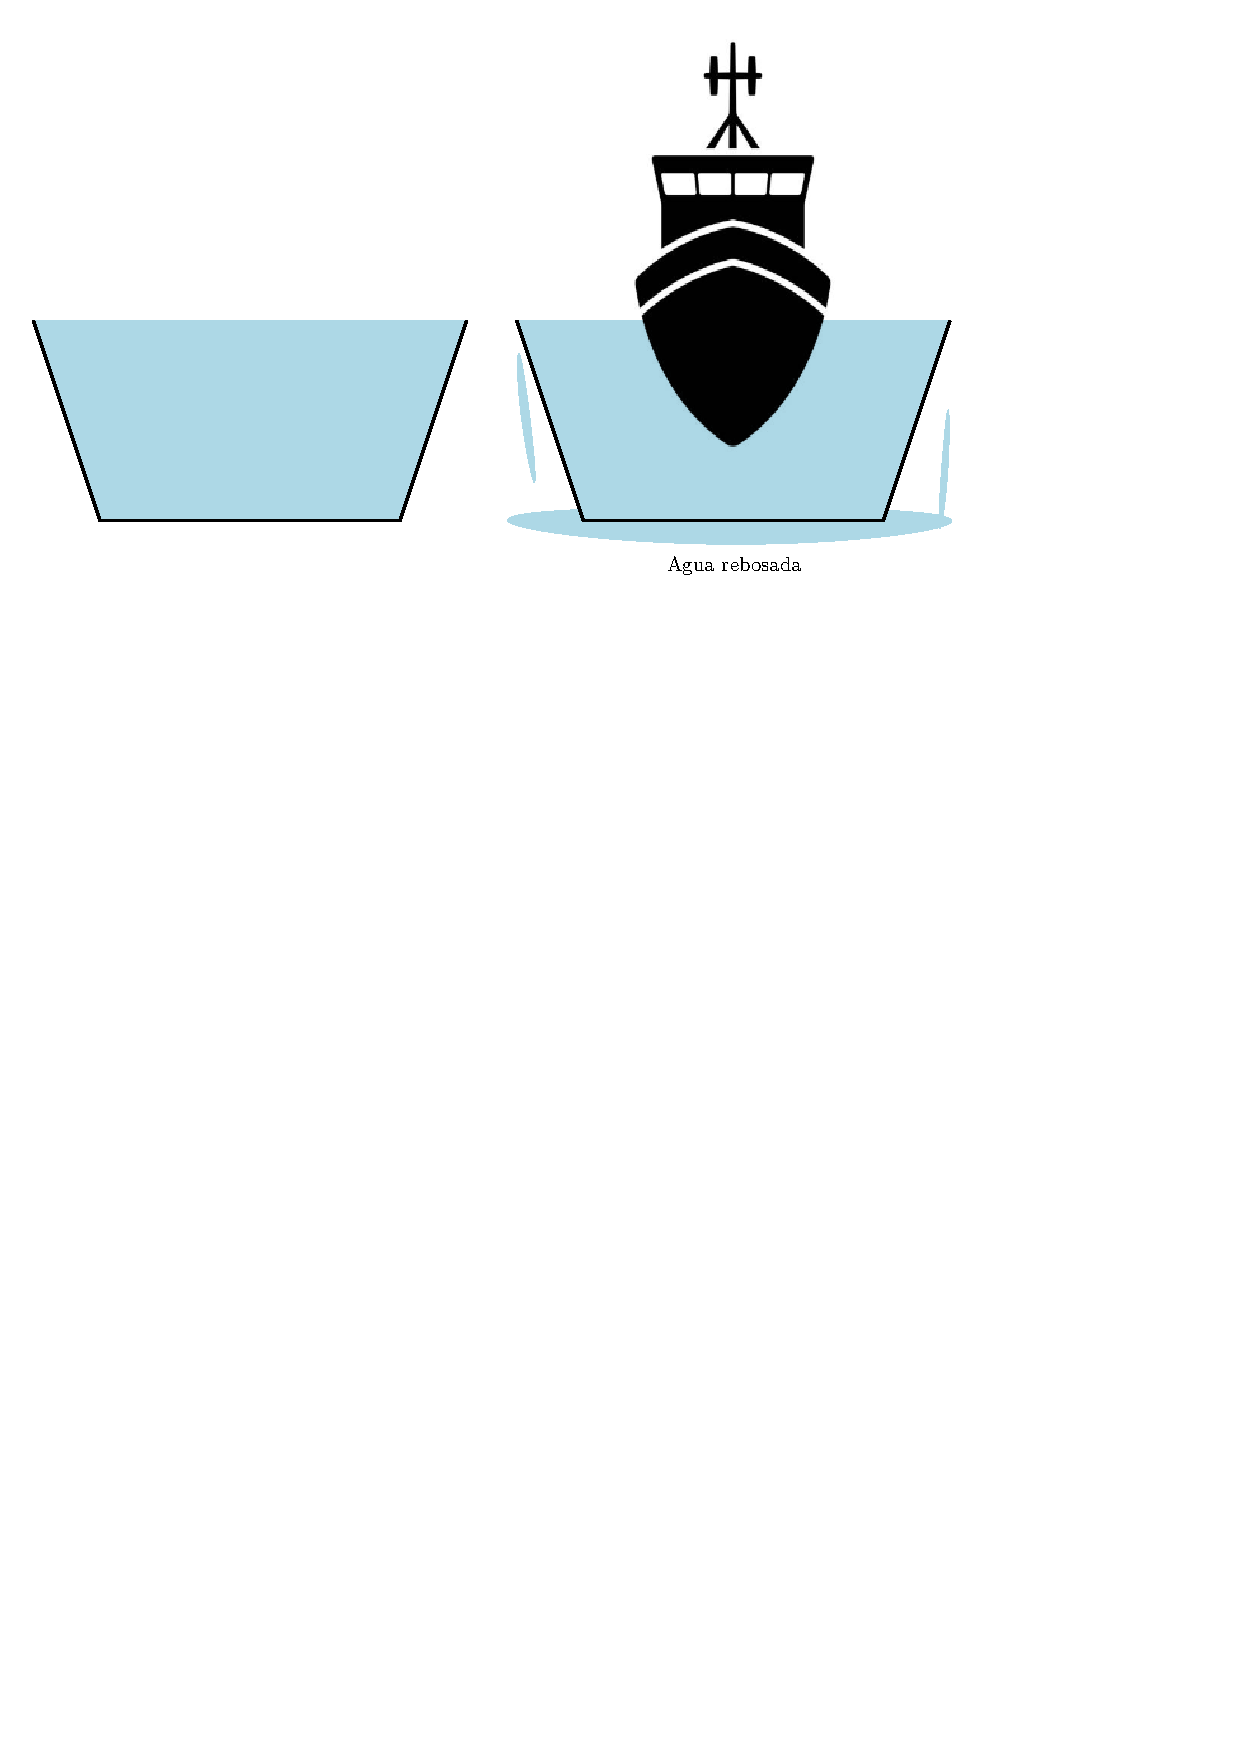
\includegraphics[width=0.75\columnwidth]{TeX_files/chapter02-Hidrostatica/arquimedes1}
	\end{center}


\section{Estabilidad}

Para un cuerpo sumergido, el centro de gravedad puede ser diferente del centro de empuje, y esto produce un momento que puede ser restaurador (equilibrio estable) o de vuelco (equilibrio inestable)

\begin{center}
	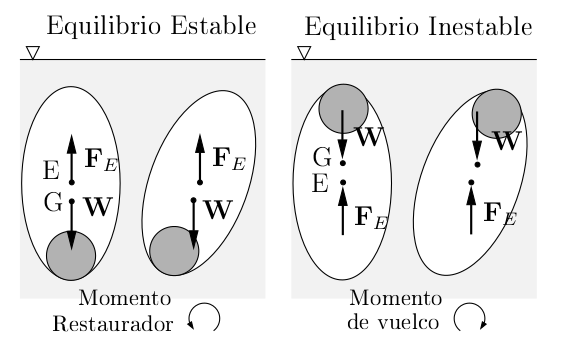
\includegraphics[width=0.7\linewidth]{TeX_files/chapter02-Hidrostatica/estabilidad1}
\end{center}

%\begin{center}
%	\includegraphics[width=0.7\columnwidth]{estab1.png}
%	% estab1.png: 996x491 pixel, 72dpi, 35.14x17.32 cm, bb=
%\end{center}


Para un cuerpo flotante, es m\'as complicado, ya que la posici\'on del centro de empuje var\'ia


Equilibrio estable 
\begin{center}
	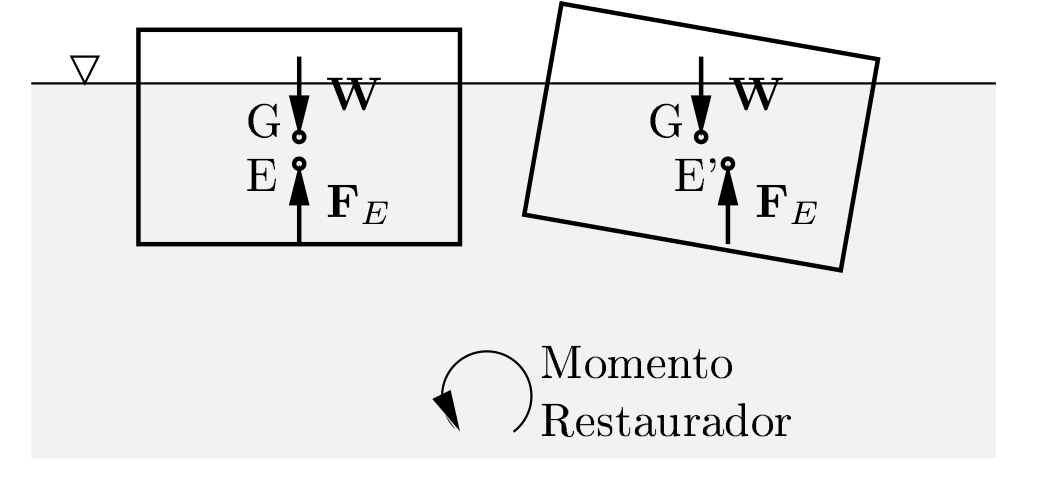
\includegraphics[width=0.7\linewidth]{TeX_files/chapter02-Hidrostatica/estabilidad2}
\end{center}



Equilibrio inestable
\begin{center}
	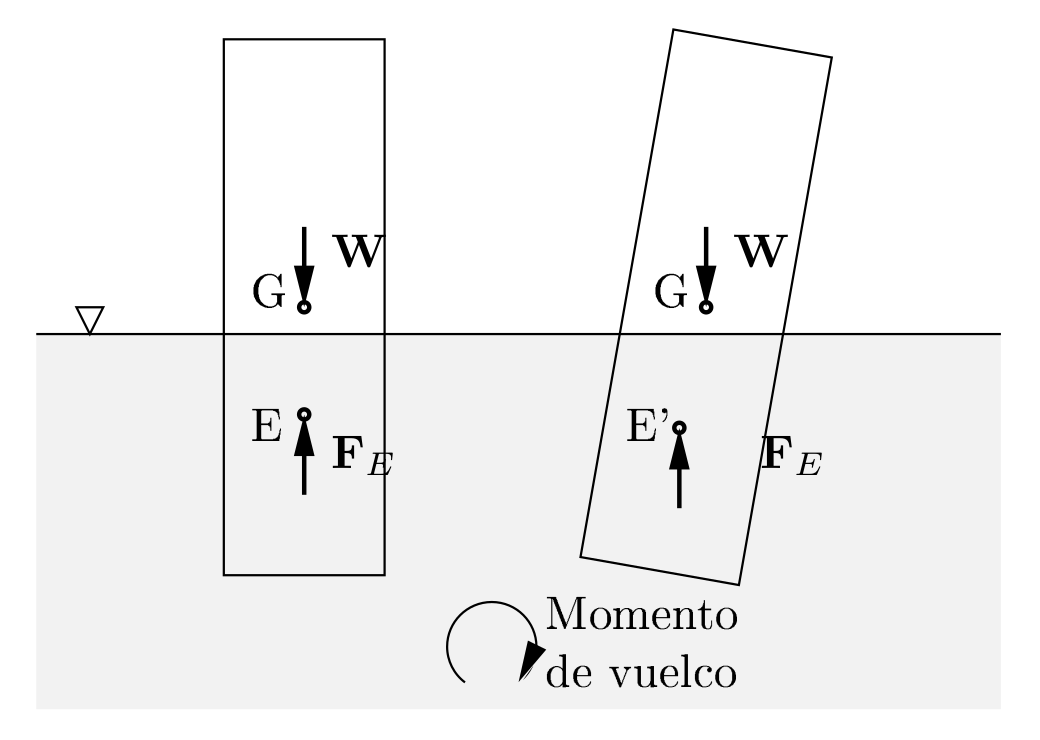
\includegraphics[width=0.7\linewidth]{TeX_files/chapter02-Hidrostatica/estabilidad3}
\end{center}


Pasos para calcular la estabilidad de un cuerpo flotante, consideremos un cuerpo sim\'etrico:

1.- Se calcula posici\'on de equilibrio inicial, mediante las fuerzas $\vec F_E$ y $\vec W$, y sus puntos de aplicaci\'on, $E$ y $G$. Como el cuerpo estan en equilibrio, estas fuerza se alinean con el eje de simetria.

2.- Se realiza una peque\~na perturbaci\'on $\Delta \theta$. El centro de empuje se desplaza a una nueva posici\'on $E'$. La vertical sobre $E'$ corta el eje de simetria en un punto $M$, denominado \textbf{metacentro}. Si el \'angulo $\Delta \theta$ es peque\~no, el metacentro no depender\'a de \'el.

3.- Se calcula la \textbf{altura metac\'entrica}, que es la distancia de $M$ a $G$. Si $M$ est\'a por encima de $G$, la altura metac\'entrica  es positiva, y la posici\'on es \emph{estable}. Si est\'a por debajo, la altura metac\'entrica es negativa, y la posici\'on es \emph{inestable}.

La altua metac\'entrica es una caracter\'istica de la secci\'on transversal del cuerpo y su distribuci\'on de masa.

\begin{center}
	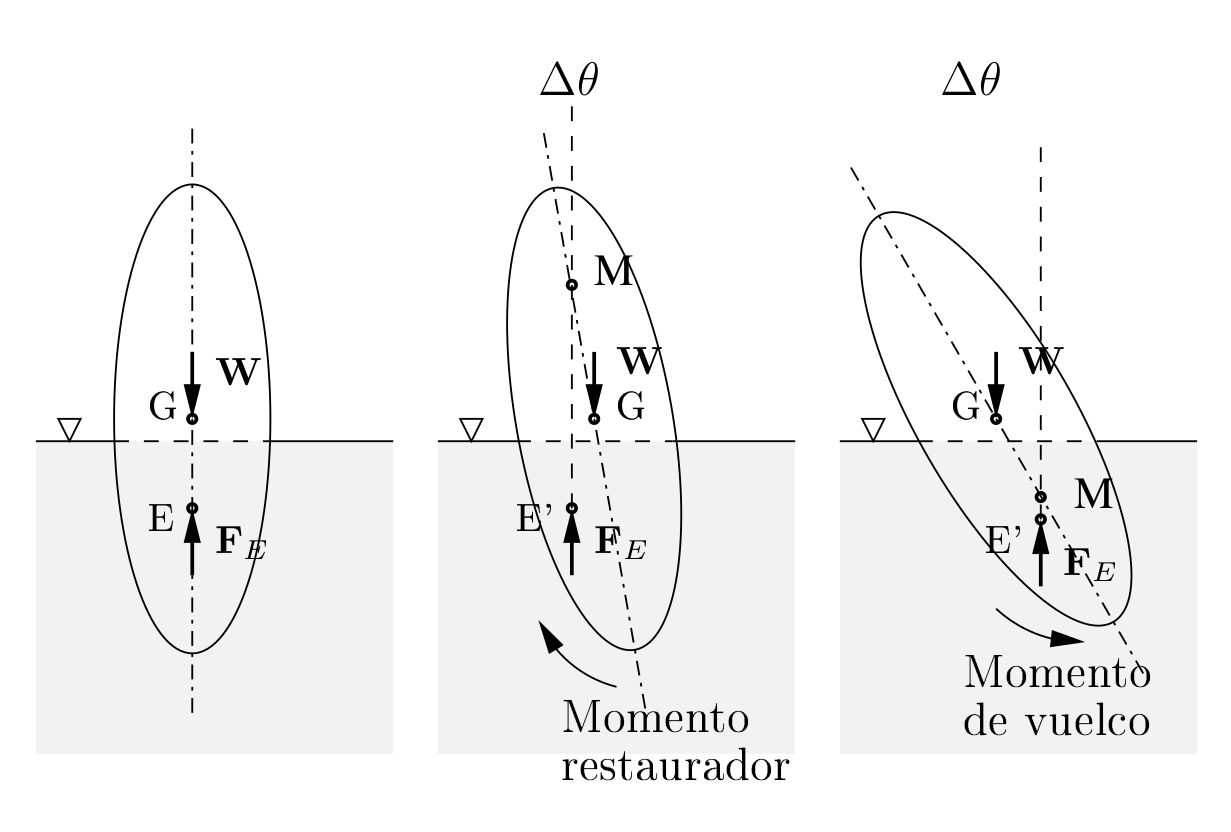
\includegraphics[width=0.7\linewidth]{TeX_files/chapter02-Hidrostatica/estabilidad4}
\end{center}

\begin{center}
	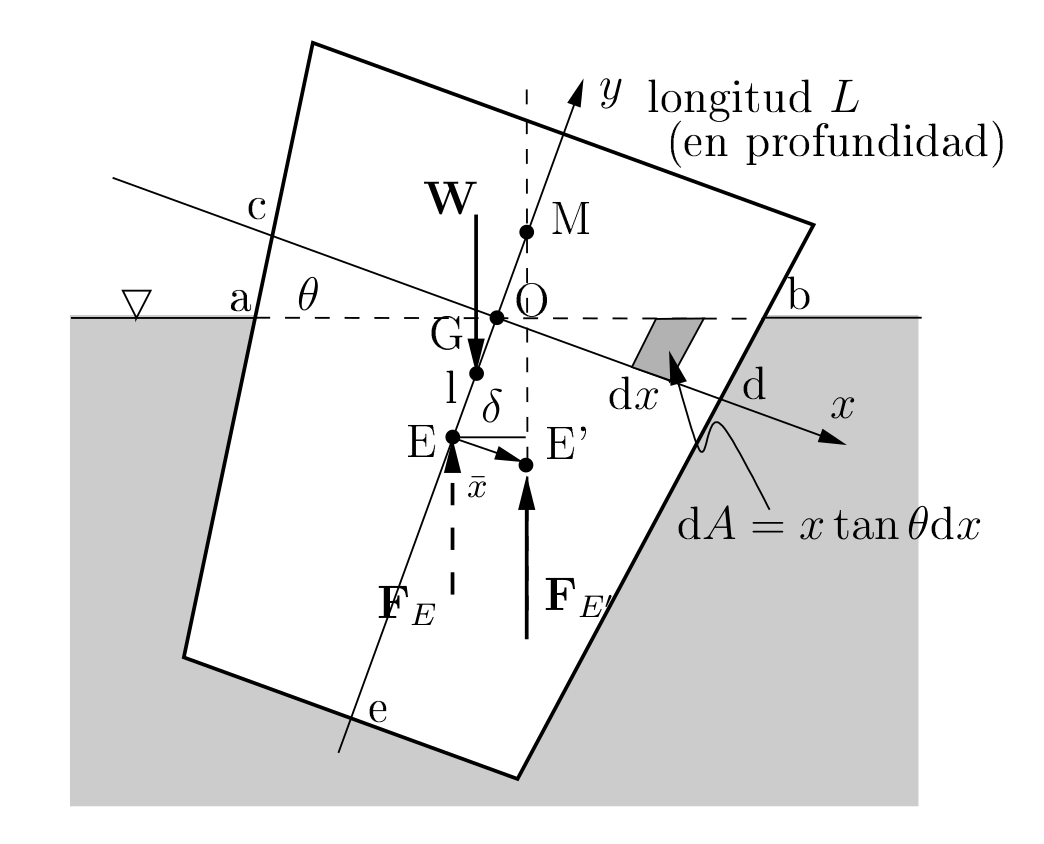
\includegraphics[width=0.7\linewidth]{TeX_files/chapter02-Hidrostatica/estabilidad5}
\end{center}




	La posici\'on del nuevo centro de empuje se calcula con la estimación del centro de masas:

\begin{align*}
	\overline{x}V_{aObdea} &= \int_{Obd}x \dif V - \int_{cOa} x \dif V
\\
	&= \int_{Obd} x L \dif A - \int_{cOa} x L \dif A 
\\
	&= \int_{Obd} x L (x\tan \theta \dif x) - \int_{cOa} x L  (-x\tan \theta \dif x)
\\
	&= \tan \theta \int x^2 2 L \dif x = \tan \theta \int x^2 \dif A 
	\\
	&= \tan \theta I_0
\end{align*}


La altura metac\'entrica es

\begin{equation}
	\overline{MG} = \overline{ME}-\overline{GE}= \frac{\overline{x}}{\tan \theta} - \overline{GE} 
= \frac{I_0}{V_{\textrm{sumergido}}} - \overline{GE} = \frac{\rho g I_0}{W} - \overline{GE}
\end{equation}

Si $\overline{MG}$ es positiva, el equilibrio es estable (para peque\~nas perturbaciones). Si 
$\overline{GE}$ es negativa, el equilibrio es estable siempre
\chapter{Cinemática de fluidos}
\section{Descripción Euleriana y Lagrangiana}
	
	Dos formas de identificación de las magnitudes (p. e., la velocidad) 
	\begin{enumerate}
		\item {\textbf{\textcolor{red}{Euleriana}}: \\
			Segun la \textcolor{blue}{posición} y el instante. 
		\begin{equation}
			\vec{u}(\vec{x},t)
		\end{equation}
		} 
		\item {\textbf{\textcolor{red}{Lagrangiana}}:\\
			Según la \textcolor{blue}{partí cula} y el instante. La partí cula
			queda identificada (marcada) mediante un vector $\vec{a}$ que puede
			ser, por ejemplo, la posición que tiene la partí cula en un instante
			de referencia $t_{0}$ 
			
\begin{equation}
				\vec{u}(\vec{a},t;t_{0})
\end{equation}
			
		} 
	\end{enumerate}


\section{Lineas de corriente, trayectorias y lineas de traza}

	
	\begin{itemize}
		\item \textcolor{red}{Lineas de corriente}:\\
		Para un instante dado $t_0$, és la tangente a los vectores de velocidad. 
	\end{itemize}

\begin{center}
	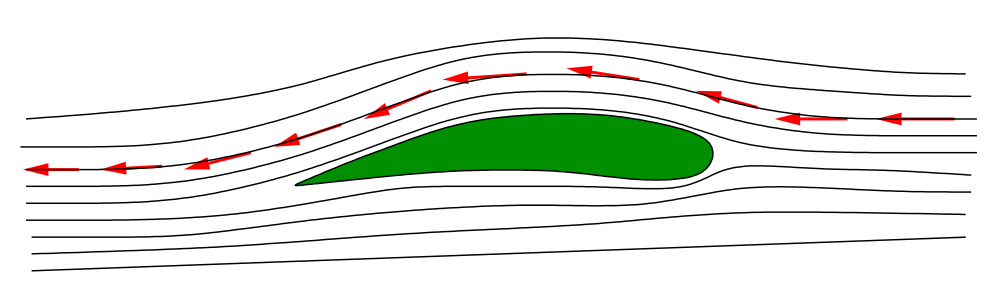
\includegraphics[width=0.7\linewidth]{TeX_files/chapter03-Cinematica/lineasCorriente}
\end{center}

		
		Són solución de la ecuación (en 2D) 
		
		\begin{equation}
			\frac{\text{d}x}{u(\vec{x},t=t_0)}=\frac{\text{d}y}{v(\vec{x},t=t_0)}
		\end{equation}
		


	
	\begin{itemize}
		\item \textcolor{red}{Trayectoria}:\\
		Para una cierta partícula de fluido, puntos que ocupa en un cierto
		intervalo de tiempo. 
		\item \textcolor{red}{Lineas de traza}:\\
		Partículas de fluido que, en un cierto instante anterior, pasaron
		por un determinado punto.
	\end{itemize}
\begin{center}
	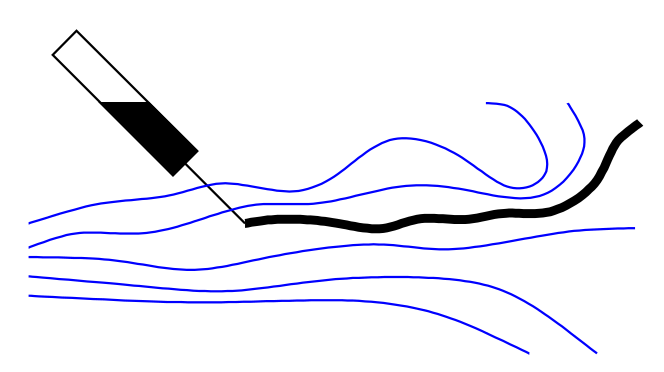
\includegraphics[width=0.5\linewidth]{TeX_files/chapter03-Cinematica/traza}
\end{center}


		
		Si el flujo es estacionario (no depende del tiempo), linea de corriente,
		trayectoria y linea de traza coinciden para un determinado punto. 
		



	
\subsection*{Actividad 1:}
		Dado el campo de velocidades bidimensional $\vec{u}=(x+t)\vec{\imath}+y\vec{\jmath}$,
		encontrad las expresiones para:
		
		a) la linea de corriente que pasa por $(1,1)$ para $t=0$
		
		b) la trayectoria de la partícula que está en $(1,1)$ para $t=0$
		
		c) la línea de traza, para $t=0$, de todas las partículas que pasaron
		por $(1,1)$


\section{Derivada sustancial}

	
	La partícula $P$, en el instante $t$ se encuentra en $\vec{x}$
	con una velocidad $\vec{u}$. La aceleración de $P$ \textbf{no} és
	$\dparc{\vec{u}}{t}$, ya que aunque $\vec{u}$ sea estacionario,
	$P$ puede estar moviéndose a un punto en que $\vec{u}$ és diferente.
	
	En un instante $t+\delta t$, $P$ estará en $\vec{x}+\delta\vec{x}=\vec{x}+\vec{u}\delta t$,
	de forma que la variación de velocidad será 
	\[
	\delta\vec{u}=\vec{u}(\vec{x}+\vec{u}\delta t,t+\delta t)-\vec{u}(\vec{x},t)
	\]
	
	Desarrollando en serie de Taylor hasta primer orden, obtenemos 
	\[
	\delta\vec{u}=\dparc{\vec{u}}{t}\delta t+(\vec{u}\cdot\vec{\nabla})\vec{u}\delta t+O(\delta t^{2}),
	\]
	de forma que la aceleración és 
	\[
	\vec{a}(\vec{x},t)=\dparc{\vec{u}}{t}+(\vec{u}\cdot\vec{\nabla})\vec{u}
	\]
	

De forma general, consideremos cualquier magnitud $f$, asociada a
una propiedad del fluido (puede ser un escalar como la temperatura,
o densidad, o la velocidad angular). 
\begin{itemize}
	\item Derivada \textcolor{red}{local}: 
	\[
	\dparc{f}{t}
	\]
	
	\item Derivada \textcolor{red}{convectiva}: 
	\[
	(\vec{u}\cdot\vec{\nabla})\vec{f}=\left(u\dparc{\phantom{f}}{x}+v\dparc{\phantom{f}}{y}+w\dparc{\phantom{f}}{z}\right)f=u_{i}\dparc{f}{x_{i}}
	\]
	
	\item Derivada \textcolor{red}{sustancial} o \textcolor{red}{total}: 
	\[
	\frac{\text{D}f}{\text{D}t}=\dparc{f}{t}+(\vec{u}\cdot\vec{\nabla})\vec{f}=\dparc{f}{t}+u_{i}\dparc{f}{x_{i}}
	\]
	
\end{itemize}

\section{Circulación, Flujo y Vorticidad}

	
	\begin{itemize}
		\item \textbf{\textcolor{red}{Circulación}}\\
		
		\[
		\Gamma=\oint_{L}\vec{u}\cdot\text{d}\vec{l}
		\]
		$L$ es cualquier contorno cerrado.
	\end{itemize}
	Si este contorno está constituido siempre por las mismas partí culas
	(es decir, es una línea material), se puede demostrar (\cite{Vir1})
	que 
	\[
	\Deriv{\Gamma}{t}=\Deriv{\phantom{t}}{t}\oint_{L}\vec{u}\cdot\text{d}\vec{l}=0
	\]
	

	
	\begin{itemize}
		\item \textbf{\textcolor{red}{Flujo}}\\
		Sea $F$ una magnitud extensiva propiedad del fluido y $f$ esta
		misma magnitud por unidad de volumen. El flujo de $f$ a través de
		la superficie $S$ es
	\end{itemize}
	\[
	\Phi=\int_{S}f\vec{u}\cdot\text{d}\vec{S}
	\]
	Si $f$ es un escalar, $f\vec{u}$ es el \textcolor{blue}{vector
		flujo} de $f$.
	
	Si $f$ es un vector $\left(\vec{f}\right)$ , $\vec{f}\vec{u}$ es
	el \textcolor{blue}{tensor flujo} de $f$.

	
{Ejemplo:}
		
		\[
		f=1\rightarrow\begin{cases}
			\vec{u} & \textrm{vector flujo volumétrico}\\
			Q=\int_{S}\vec{u}\cdot\text{d}\vec{S} & \textrm{flujo volumétrico, o caudal}
		\end{cases}
		\]
		
		\[
		f=\rho\rightarrow\begin{cases}
			\rho\vec{u} & \textrm{vector flujo másico}\\
			\dot{m}=\int_{S}\rho\vec{u}\cdot\text{d}\vec{S} & \textrm{flujo másico, o gasto}
		\end{cases}
		\]
		

\begin{itemize}
	\item \textbf{\textcolor{red}{Vorticidad}}\\
	
	\[
	\vec{\omega}=\vec{\nabla}\times\vec{u}\quad\text{En componentes:}\quad\omega_{k}=-\varepsilon_{ijk}\dparc{u_{i}}{x_{j}}
	\]
	Es el doble de la velocidad local de rotación del elemento de fluido.
	Por definición de vorticidad, se cumple que 
	\[
	\vec{\nabla}\cdot\vec{\omega}=0
	\]
	y el flujo a través de una superficie $S$ cerrada es siempre nulo
	\[
	\oint_{S}\vec{\omega}\cdot\text{d}\vec{S}=0
	\]
	\item Si la superficie es abierta, este flujo está relacionado con la circulación
	sobre la línea que limita la superficie a través del Teorema de Stokes
	\[
	\int_{S}\vec{\omega}\cdot\text{d}\vec{S}=\int_{S}\left(\vec{\nabla}\times\vec{u}\right)\cdot\text{d}\vec{S}=\oint_{L}\vec{u}\cdot\text{d}\vec{l}
	\]
	
\end{itemize}

\section{Movimiento relativo en el entorno de un punto}

	
	Sea $\vec{u}$ la velocidad del fluido en un punto $\vec{r}$. En
	un punto $\vec{r}+\delta\vec{r}$, la velocidad será $\vec{u}+\delta\vec{u}$,
	con 
	\[
	\delta\vec{u}=\vec{\nabla}\vec{u}\cdot\delta\vec{r};\ \delta u_{i}=\dparc{u_{i}}{x_{j}}\delta r_{j}
	\]
	
	El tensor \textcolor{blue}{divergencia de velocidad}, $\vec{\nabla}\vec{u}$,
	puede descomponerse como la suma de un tensor simétrico,$\left(\vec{\nabla}\vec{u}\right)^{S}$
	y un tensor antisimétrico $\left(\vec{\nabla}\vec{u}\right)^{A}$,
	con 
	\begin{eqnarray*}
		\left(\vec{\nabla}\vec{u}\right)^{S}=\frac{1}{2}\left(\vec{\nabla}\vec{u}+\left(\vec{\nabla}\vec{u}\right)^{T}\right)\\
		\left(\vec{\nabla}\vec{u}\right)^{A}=\frac{1}{2}\left(\vec{\nabla}\vec{u}-\left(\vec{\nabla}\vec{u}\right)^{T}\right)
	\end{eqnarray*}
	
	Cada uno de estos tensores contribuye a $\delta\vec{u}$ de una forma
	diferente 
	\[
	\delta\vec{u}=\delta\vec{u}^{S}+\delta\vec{u}^{A}=\left(\vec{\nabla}\vec{u}\right)^{S}\cdot\delta\vec{r}+\left(\vec{\nabla}\vec{u}\right)^{A}\cdot\delta\vec{r}
	\]
	

	
	$\delta\vec{u}^{S}=\left(\vec{\nabla}\vec{u}\right)^{S}\cdot\delta\vec{r}$
	representa un movimiento de \textcolor{blue}{deformación pura}. Siempre
	es posible escoger los ejes del sistema de referencia de forma que
	$\left(\vec{\nabla}\vec{u}\right)^{S}$ sea diagonal. Entonces los
	tres valores de la diagonal son las velocidades de estiramiento en
	la dirección de los ejes principales. Si el fluido es incompresible
	el volumen del elemento de fluido se mantiene constante y la suma
	de la diagonal, que es un invariante respecto del cambio de sistema
	de coordenadas, es nula 
	\[
	\dparc{u_{i}}{x_{i}}=0
	\]
	

	
	$\delta\vec{v}^{A}=\left(\vec{\nabla}\vec{u}\right)^{A}\cdot\delta\vec{r}$
	representa un movimiento de \textcolor{blue}{rotación pura}. 
	\[
	\delta u_{i}^{A}=\frac{1}{2}\left(\dparc{u_{i}}{x_{j}}-\dparc{u_{j}}{x_{i}}\right)\delta r_{j}=\frac{1}{2}\varepsilon_{ijk}\omega_{k}\delta r_{j}
	\]
	La velocidad angular de rotación es $\frac{1}{2}\vec{\omega}=\frac{1}{2}(\vec{\nabla}\times\vec{u})$. 




\backmatter
% bibliography, glossary and index would go here.

\end{document}